% Created 2024-01-29 Mon 21:26
% Intended LaTeX compiler: pdflatex
\documentclass[11pt]{article}
\usepackage[utf8]{inputenc}
\usepackage[T1]{fontenc}
\usepackage{graphicx}
\usepackage{longtable}
\usepackage{wrapfig}
\usepackage{rotating}
\usepackage[normalem]{ulem}
\usepackage{amsmath}
\usepackage{amssymb}
\usepackage{capt-of}
\usepackage{hyperref}
\usepackage{minted}
\usepackage{xcolor}
\usepackage{tcolorbox}
\usepackage{biblatex}
\author{Nidish Balaji}
\date{2024:Jan:17}
\title{Implementation and Validation of the Fokker-Planck Equation for Narrow-band excitation}
\hypersetup{
 pdfauthor={Nidish Balaji},
 pdftitle={Implementation and Validation of the Fokker-Planck Equation for Narrow-band excitation},
 pdfkeywords={},
 pdfsubject={},
 pdfcreator={Emacs 29.1 (Org mode 9.6.6)}, 
 pdflang={English}}
\makeatletter
\newcommand{\citeprocitem}[2]{\hyper@linkstart{cite}{citeproc_bib_item_#1}#2\hyper@linkend}
\makeatother

\usepackage[notquote]{hanging}
\begin{document}

\maketitle

\section{Week 1}
\label{sec:orgd48771b}
\subsection{Excitation Design (from \citeprocitem{1}{[1]})}
\label{sec:orgccc7715}
\begin{itemize}
\item The excitation is designed through the stochastically defined phase \(\sigma(t)\),
$$ d\sigma = \frac{\Omega}{F_s} dt + \frac{\nu}{F_s} dW, $$
where \(W(t)\) is the unit Wiener process (\(dW=\eta\sim\mathcal{N}(0,1)\)), and \(F_s\) is the sampling rate (in Hz).
\item The excitation signal is then written as
$$ f(t) = F \cos\sigma(t), $$
where \(F\) is the excitation amplitude.
\item Theoretically, the spectrum this leads to is
$$ \Phi_{FF}(\omega) = \frac{\lambda^2\overline{\nu}^2}{4\pi}
  \frac{\overline{\Omega}^2+\frac{\overline{\nu}^4}{4}+\omega^2}{(\Omega^2+\frac{\overline{\nu}^4}{4}-\omega^2)^2+\omega^2\overline{\nu}^4}\text{,
    with } \overline{\nu}=\frac{\nu}{\sqrt{F_s}}.  $$
\item Here is an example of the averaged spectrum with \(\Omega=100\,rad/s\), \(\nu=5\sqrt{F_s}\,rad/s\), and \(F_s=1024\,Hz\). The -3dB bandwidth of the signal is \({(\nu/\sqrt{F_s})}^2\, rad/s\), that is also indicated in the figure.
\begin{figure}[htbp]
\centering
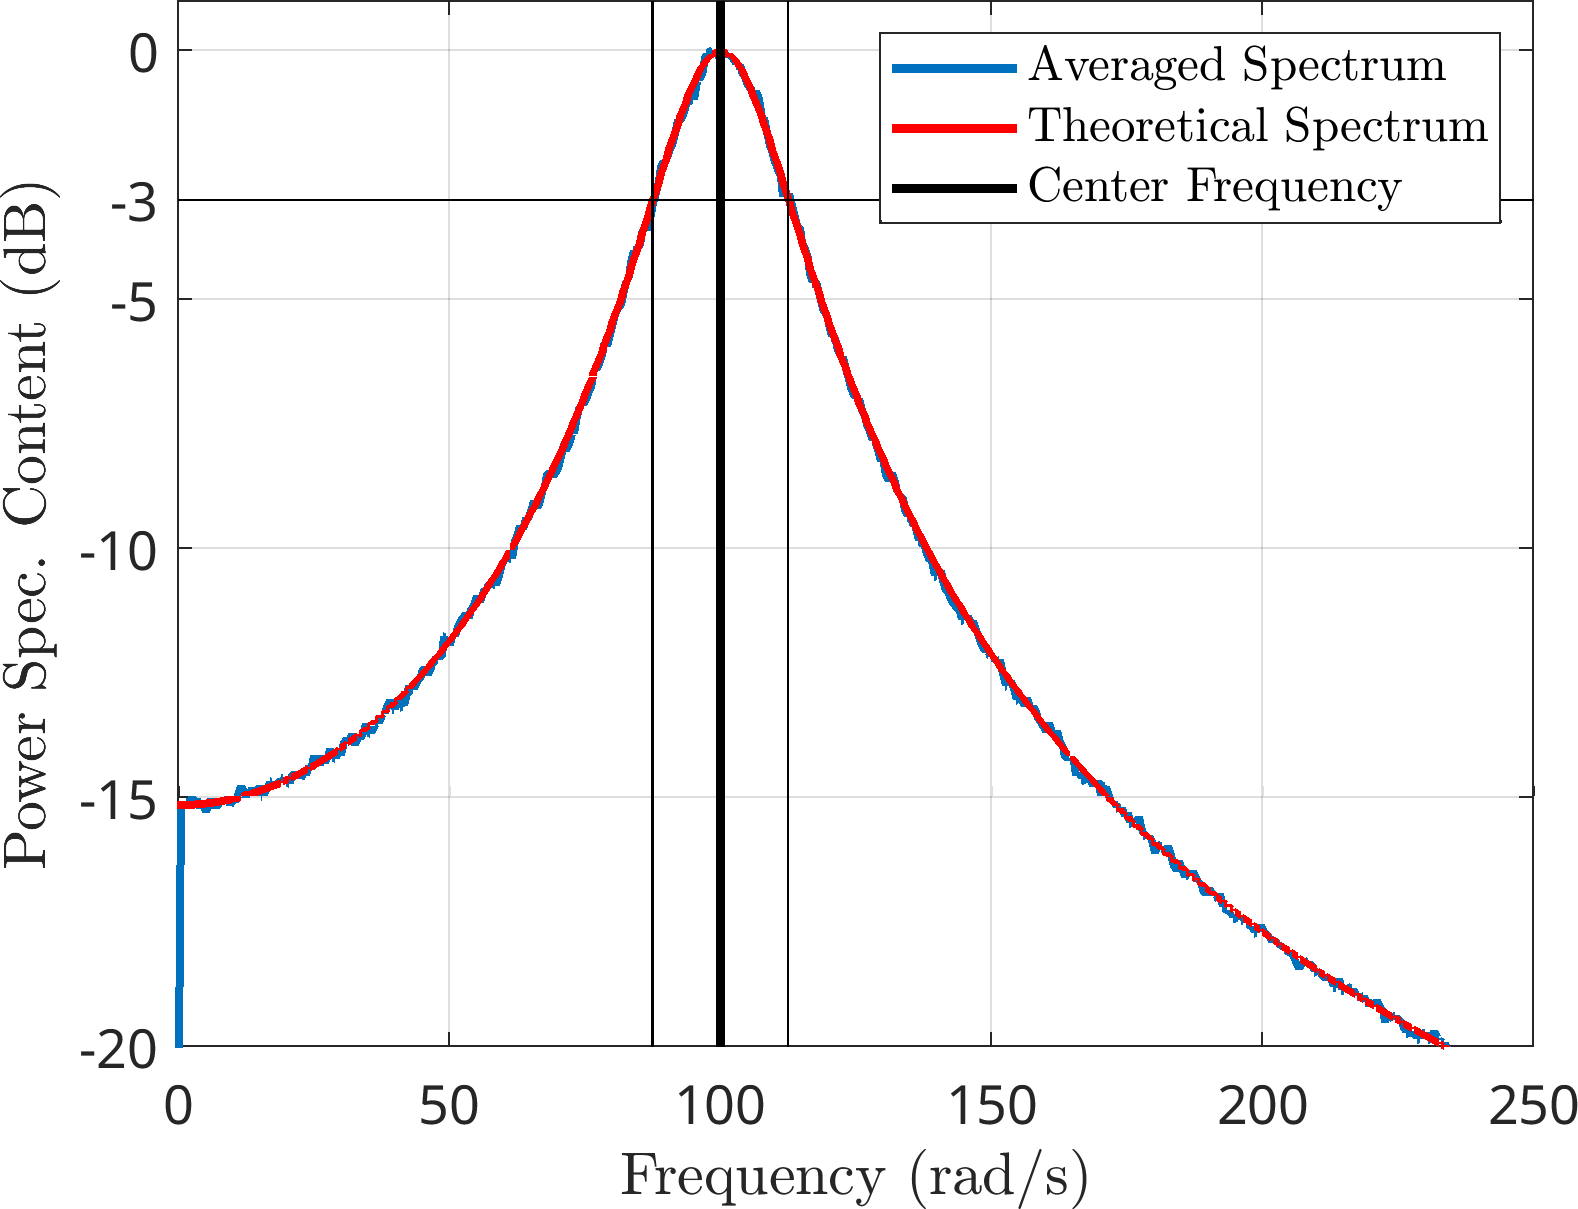
\includegraphics[width=.9\linewidth]{./FIGS/B_AvSpec.png}
\caption{\label{avspec}Averaged excitation spectrum along with the theoretical spectrum}
\end{figure}
\item Here is a single realization of the same signal. 
\begin{figure}
\begin{figure}[htbp]
\centering
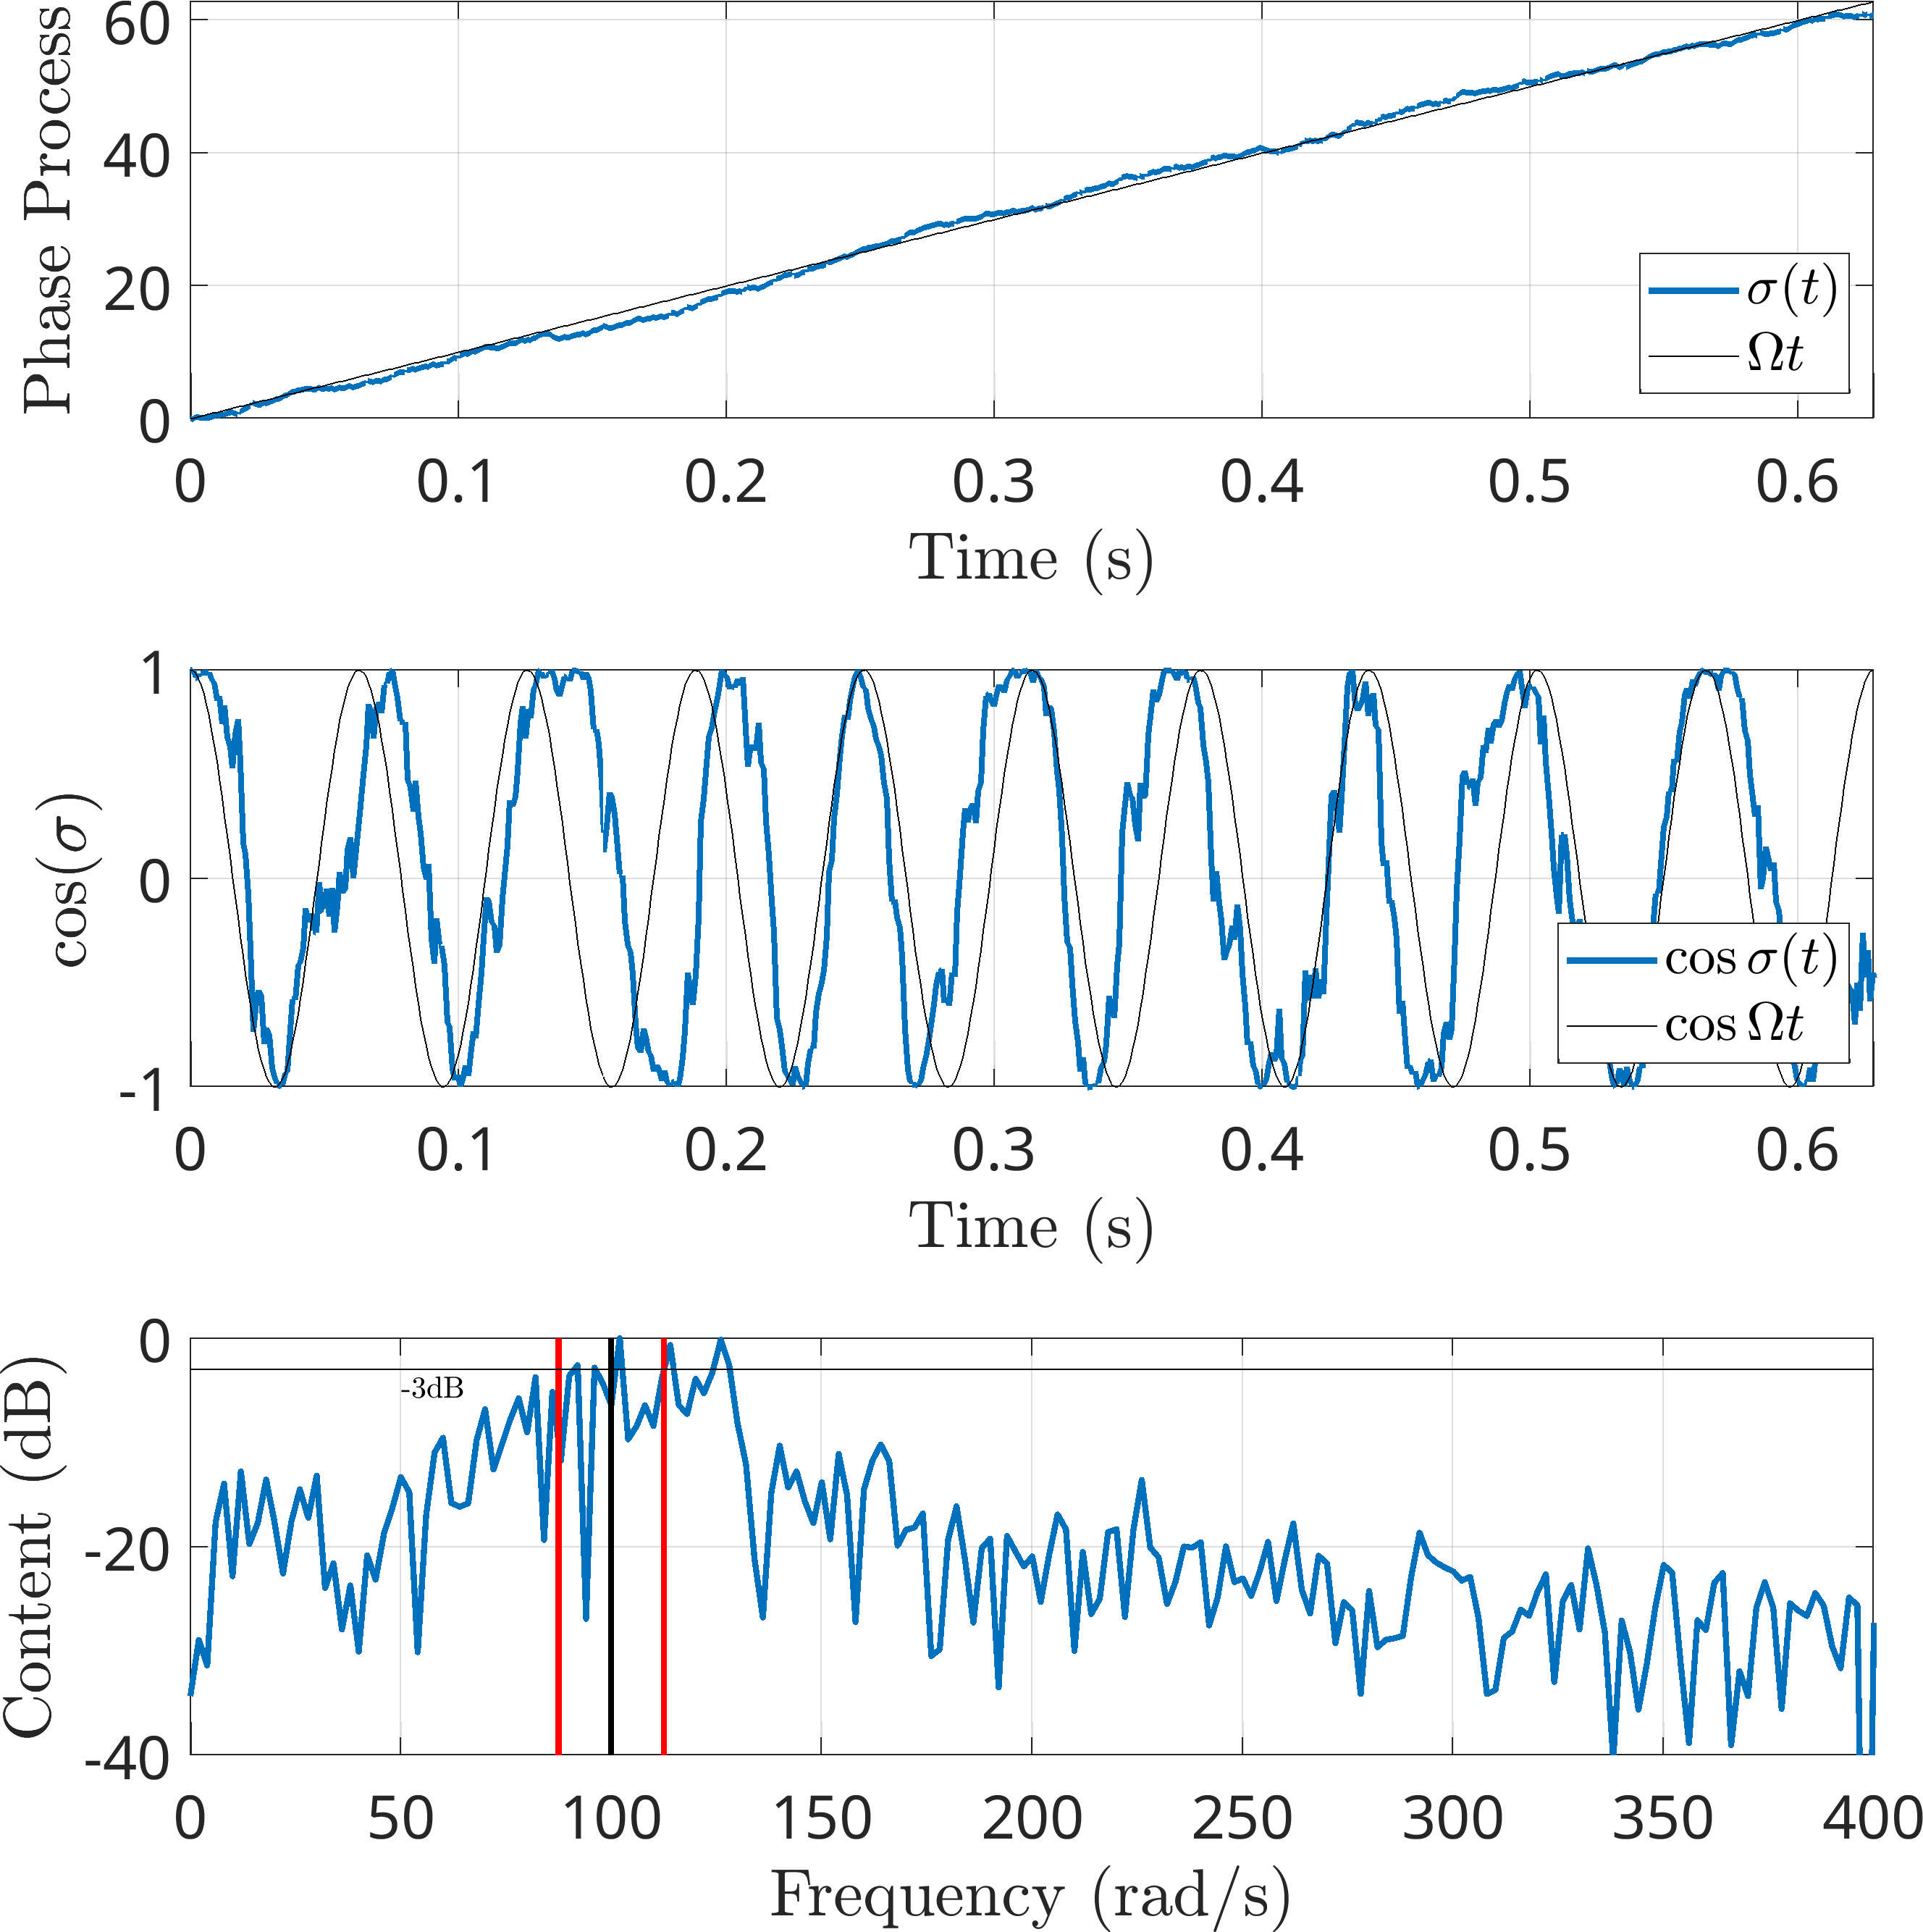
\includegraphics[width=.9\linewidth]{FIGS/B_NBsig.png}
\caption{Single Realization of Excitation Signal}
\end{figure}      
\label{real}
\end{figure}
\end{itemize}
\subsection{Stochastic Dynamics Overview + FPE}
\label{sec:org48d9278}
\begin{itemize}
\item Consider a first order dynamical system of the form,
$$ \dot{x}^{(n)} = f(t,x) + h(t,x)\dot{w}^{(n)(t)}. $$
\item We are interested in the case when the excitation term \(w^{(n)}(t)\) is an \textbf{approximation of a stochastic process} where \(n\) (sampling rate) is chosen such that it converges to the unit Wiener process, \(w(t)\), as \(n\to \infty\).
\item Ref. \citeprocitem{2}{[2]} showed that this converges, as \(n\to\infty\), to the Itô SDE given by,
$$ dx_t = \frac{1}{F_s} \left(f(t,x_t)+\frac{1}{2F_s} \nabla_x h(t,x_t) h(t,x_t)\right) dt + \frac{1}{F_s} h(t,x_t)dW_t. $$
\begin{itemize}
\item In tensor notation, this is,
$$ {dx_t}_i = \frac{1}{F_s}\left( f_i(t,x_t) + \frac{1}{2F_s} \frac{\partial
        h_i(t,x_t)}{\partial x_j}h_j(t,x_t)\right) dt + \frac{1}{F_s}h_i(t,x_t)
    dW_t $$
\end{itemize}
\item This is rewritten (for convenience) as
$$ dx_t = \mu(t,x_t)dt + \sigma(t,x_t)dW, $$
where \(\mu,\sigma:\mathbb{R}\times\mathbb{R}^d\to \mathbb{R}^d\), with \(d\) being the number of states \(x\).
\item The diffusion of probability of this SDE is governed by the Fokker-Planck Equation (FPE) or Fokker-Planck-Kolmogorov forward equation,
$$ \dot{p} + J_{i,i}=0,\,\text{with }J_i=\mu_ip-\frac{1}{2}(\sigma_i\sigma_j
  p)_{,j},\,\text{such that, }\int_{\mathcal{D}}p=1, $$
where \(\mathcal{D}\) is the domain of \(x_t\).
\item \(p(x)\) is the \textbf{probability density} and \(J_i(x)\) is the \textbf{probability flux}.
\item Two kinds of boundary conditions (on faces) are possible for the PDE:
\begin{enumerate}
\item \emph{Absorbing}: \(p=0\).
\item \emph{Reflecting}: \(J_i n_i=0\)
\end{enumerate}
\end{itemize}

\subsubsection{Weak form of the FPE}
\label{sec:orgdde7388}
\begin{itemize}
\item The weak form of the FPE is written as follows, denoting the domain by \(\mathcal{D}\) and using a trial function \(g:\mathcal{D}\to\mathcal{H}\) (with \(\mathcal{H}\) satisfying Dirichlet B.C.s),
\begin{align*}
  G(g,p) &= \int_{\mathcal{D}} g \dot{p} + \int_{\mathcal{D}} gJ_{i,i}\\
         &= \int_{\mathcal{D}} g \dot{p} - \int_{\mathcal{D}} g_{,i}J_i + \int_{\partial \mathcal{D}} g J_in_i,
\end{align*}
where \(\partial \mathcal{D}\) denotes the boundary and \(n_i\) denotes the relevant boundary normal.
\begin{itemize}
\item The symbol \(\int_{\mathcal{D}} g p\) denotes some inner product defined over the domain \(\mathcal{D}\).
\end{itemize}
\item On \emph{absorbing} boundaries, \(g\) will be chosen to be 0 (since \(p=0\)), so the boundary term will be zero.
\item On \emph{reflecting} boundaries, the probability flux, \(J_i n_i\), will be 0, so here, too, the boundary term cancels out.
\item Using a discretization for \(p\) in the form,
$$ p = \mathbf{N}_k(x) \hat{p}_k(t), $$
and applying a Galerkin projection (choosing \(N_k(x)\) as \(g(x)\)) yields the following matrix form of the governing equations
$$ \left[\int_\mathcal{D} \mathbf{N}_k \mathbf{N}_l\right] \hat{p}_l - \left[\int_{\mathcal{D}}
  \mathbf{N}_{k,i}(\mu_i-\frac{1}{2}(\sigma_i\sigma_j)_{,j}) \mathbf{N}_l -
  \frac{1}{2} \int_{\mathcal{D}} \mathbf{N}_{k,i} (\sigma_i\sigma_j) \mathbf{N}_{l,j}\right]
  \hat{p} = 0. $$
\item The probability constraint can be written as \(\left( \int_{\mathcal{D}}\mathbf{N}_k \right) \hat{p} = 1\).
\item The above presents a homogeneous system of ODE written as
$$ \mathbf{M} \dot{\hat{p}} - \mathbf{K} \hat{p} = 0,\,\text{s.t., }
  T \hat{p}=1. $$
\item \textbf{Steady-solutions may be obtained using eigenanalysis of the GEVP \(\left(\mathbf{K}-\lambda\mathbf{M}\right) \phi = 0\)}
\item The other approaches in the literature include \citeprocitem{3}{[3]}, \citeprocitem{4}{[4]}
\item Assessing the leading eigenpair, two cases arise:
\begin{itemize}
\item \(\lambda_1=0\): Corresponds to a \textbf{Stationary Process} at steady-state..
\item \(\Re\{\lambda_1\}=0,\,\Im\{\lambda_1\}\neq0\): Corresponds to a \textbf{Periodic random process} at steady-state.
\end{itemize}
\end{itemize}

\subsection{Slow-Flow Amplitude-Phase Dynamics}
\label{sec:org1329c33}
\begin{itemize}
\item The modal equations of motion of a nonlinear oscillator can be expressed as,
$$ \ddot{x} + 2\zeta\omega_0 \dot{x} + \omega_0^2 x = \frac{F}{2} e^{j\sigma} + c.c., $$
where \(\zeta,\, \omega_0\), and \(F\) are real-valued functions of a slowly-evolving amplitude \(q\).
\begin{itemize}
\item In the MDOF nonlinear context, NMA provides \(\zeta\)(q), \(\omega_0(q)\), and \(\psi(q)\).
\item The excitation can be expressed as \(F(q) = |\psi(q)^H f|\), where \(f\) is the forcing vector of the system.
\item The absolute of the \(\psi^H f\) quantity can be considered w.l.o.g. since \(\sigma\) can always be chosen to offset the phase of this complex quantity.
\end{itemize}
\item We have already seen that the dynamics of the slow-flow quantities can be derived using either
\begin{itemize}
\item \textbf{the method of multiple scales}, which starts from
$$ \ddot{x} + \textcolor{red}{\epsilon} 2\zeta\omega_0 \dot{x} + \omega_0^2 x =
    \textcolor{red}{\epsilon} \frac{F}{2} e^{j\sigma}+c.c.,\,\text{with }
    d\sigma=\omega_0 dt+\textcolor{red}{\epsilon}((\Omega-\omega_0)dt+\nu dW ), \text{, or} $$
\item \textbf{the enriched MMS}, which starts from
$$ \ddot{x} + \textcolor{red}{p} 2\zeta\omega_0 \dot{x} + \Omega^2 x +
    \textcolor{red}{p} ((\omega_0^2-\Omega^2) x) = \textcolor{red}{p} \frac{F}{2}
    e^{j\sigma}+c.c.,\text{ with, } d\sigma = \Omega dt + \textcolor{red}{p}(\nu dW).$$
\end{itemize}
\item The final equations in general, can be written in the form
$$ \begin{bmatrix} dq\\ d\beta \end{bmatrix} = \begin{bmatrix} \mu_1(q,\beta)\\
    \mu_2(q,\beta) \end{bmatrix} + \begin{bmatrix} \sigma_1(q,\beta)\\
      \sigma_2(q,\beta)\end{bmatrix} dW. $$
\item The FPE is written as above, in the semi-periodic 2D domain \(\mathcal{D}=\{x_1\in\mathbb{R}^+,\, x_2\in]-\pi,\pi[\}\).
\item The periodic boundary conditons over \(x_2=\pm\pi\) also make the boundary terms in the weak form vanish.
\item Four different cases will be considered for the studies:
\begin{center}
\begin{tabular}{rll}
\hline
1. & \textbf{MMS1} & MMS Truncated up to \(\mathcal{O}(\textcolor{red}{\epsilon})\)\\[0pt]
2. & \textbf{MMS2} & MMS Truncated up to \(\mathcal{O}(\textcolor{red}{\epsilon}^2)\)\\[0pt]
3. & \textbf{EMMS1} & EMMS Truncated up to \(\mathcal{O}(\textcolor{red}{p})\)\\[0pt]
 &  & (Same as CXA)\\[0pt]
4. & \textbf{EMMS2} & EMMS Truncated up to \(\mathcal{O}(\textcolor{red}{p}^2)\)\\[0pt]
\hline
\end{tabular}
\end{center}
\item The practical relevance of the conceptual difference of \(MMS\) and \(EMMS/CXA\) remains to be seen.
\end{itemize}

\subsubsection{Validation on Linear System Dynamics}
\label{sec:org57fbe50}
\begin{itemize}
\item For Linear systems (\(\zeta, \omega_0, F\) taken to be constants), the slow-flow expressions turn out to be,
\begin{itemize}
\item \textbf{MMS}:
\begin{align*}
  \dfrac{d}{dt} \begin{bmatrix} q\\\\\beta \end{bmatrix} =
  \left(\textcolor{red}{\epsilon} \begin{bmatrix} -\zeta \omega_0 q - \dfrac{F\sin
    \beta}{2\omega_0}\\\\-(\Omega-\omega_0)-\dfrac{F\cos \beta}{2\omega_0q} \end{bmatrix} +
  \textcolor{red}{\epsilon^2} \begin{bmatrix}\dfrac{F\zeta \cos \beta}{4\omega_0} +
    (\Omega-\omega_0)\dfrac{F\sin \beta}{4\omega_0^2}\\\\ -\dfrac{\zeta^2\omega_0}{2} - \dfrac{F\zeta\sin
    \beta}{4\omega_0q} + (\Omega-\omega_0)\dfrac{F\cos \beta}{4\omega_0^2q} \end{bmatrix}\right) +
  \nu \left(\textcolor{red}{\epsilon} \begin{bmatrix}0\\\\ -1\end{bmatrix} +
  \textcolor{red}{\epsilon^2} \begin{bmatrix}\dfrac{F\sin \beta}{4\omega_0^2}\\\\
    \dfrac{F\cos \beta}{4\omega_0^2q}\end{bmatrix}\right) \dot{W}(t) -
  \cancel{\left(\textcolor{red}{\epsilon^2} \frac{d\sigma}{dT_2}\right)}
\end{align*}
\begin{itemize}
\item Phase:
$$ \sigma = \omega_0 t + \textcolor{red}{\epsilon}(\Omega-\omega_0)t + \textcolor{red}{\epsilon} \nu W(t) $$
\end{itemize}
\item \textbf{EMMS}:
\begin{align*}
  \dfrac{d}{dt} \begin{bmatrix} q\\\\\beta \end{bmatrix} =
  \left(\textcolor{red}{p} \begin{bmatrix} -\zeta \omega_0q - \dfrac{F\sin
    \beta}{2\Omega}\\\\ -\dfrac{\Omega^2-\omega_0^2}{2\Omega}-\dfrac{F\cos \beta}{2\Omega
    q}\end{bmatrix} + \textcolor{red}{p^2} \begin{bmatrix} \dfrac{F\zeta
      \omega_0\cos \beta}{4\Omega^2}-(\Omega^2-\omega_0^2)\dfrac{F\sin \beta}{8\Omega^3}\\\\
      -\dfrac{(\Omega^2-\omega_0^2)^2}{8\Omega^3}-\dfrac{\zeta^2\omega_0^2}{2\Omega}-\dfrac{F\zeta\omega_0\sin
      \beta}{4\Omega^2q}-(\Omega^2-\omega_0^2)\dfrac{F\cos \beta}{8\Omega^3q} \end{bmatrix}\right)
+ \left( \textcolor{red}{p} \begin{bmatrix} 0\\\\ -1\end{bmatrix} +
  \textcolor{red}{p^2} \begin{bmatrix} \dfrac{F\sin \beta}{4\Omega^2}\\\\
    \dfrac{F\cos \beta}{4\Omega^2q}\end{bmatrix} \right) \dot{W}(t) -
  \cancel{\left(\textcolor{red}{p^2} \dfrac{d\sigma}{dT_2}\right)}
\end{align*}
\begin{itemize}
\item Phase:
$$ \sigma = \Omega t + \textcolor{red}{p} \nu W(t) $$
\end{itemize}
\end{itemize}
\item In both of these, the equations are expresed in the format shown above and the Wong and Zakai approach \citeprocitem{2}{[2]} is used to obtain the corresponding SDE.
\item The SDE is then used to derive the Fokker-Planck Equation, that is used for the comparisons.
\item The following properties are assumed for the linear parameters:
$$ \boxed{\omega_0=120\,rad/s,\, \zeta=0.002,\, F=2\,N,\, \Omega=100\,rad/s,\, \nu=5\sqrt{F_s}\implies \Omega _{bw}=25\,rad/s.} $$
\item Here is a summary plot. Deterministically, the MMS approaches seem to match the 
\begin{figure}
\begin{figure}[htbp]
\centering
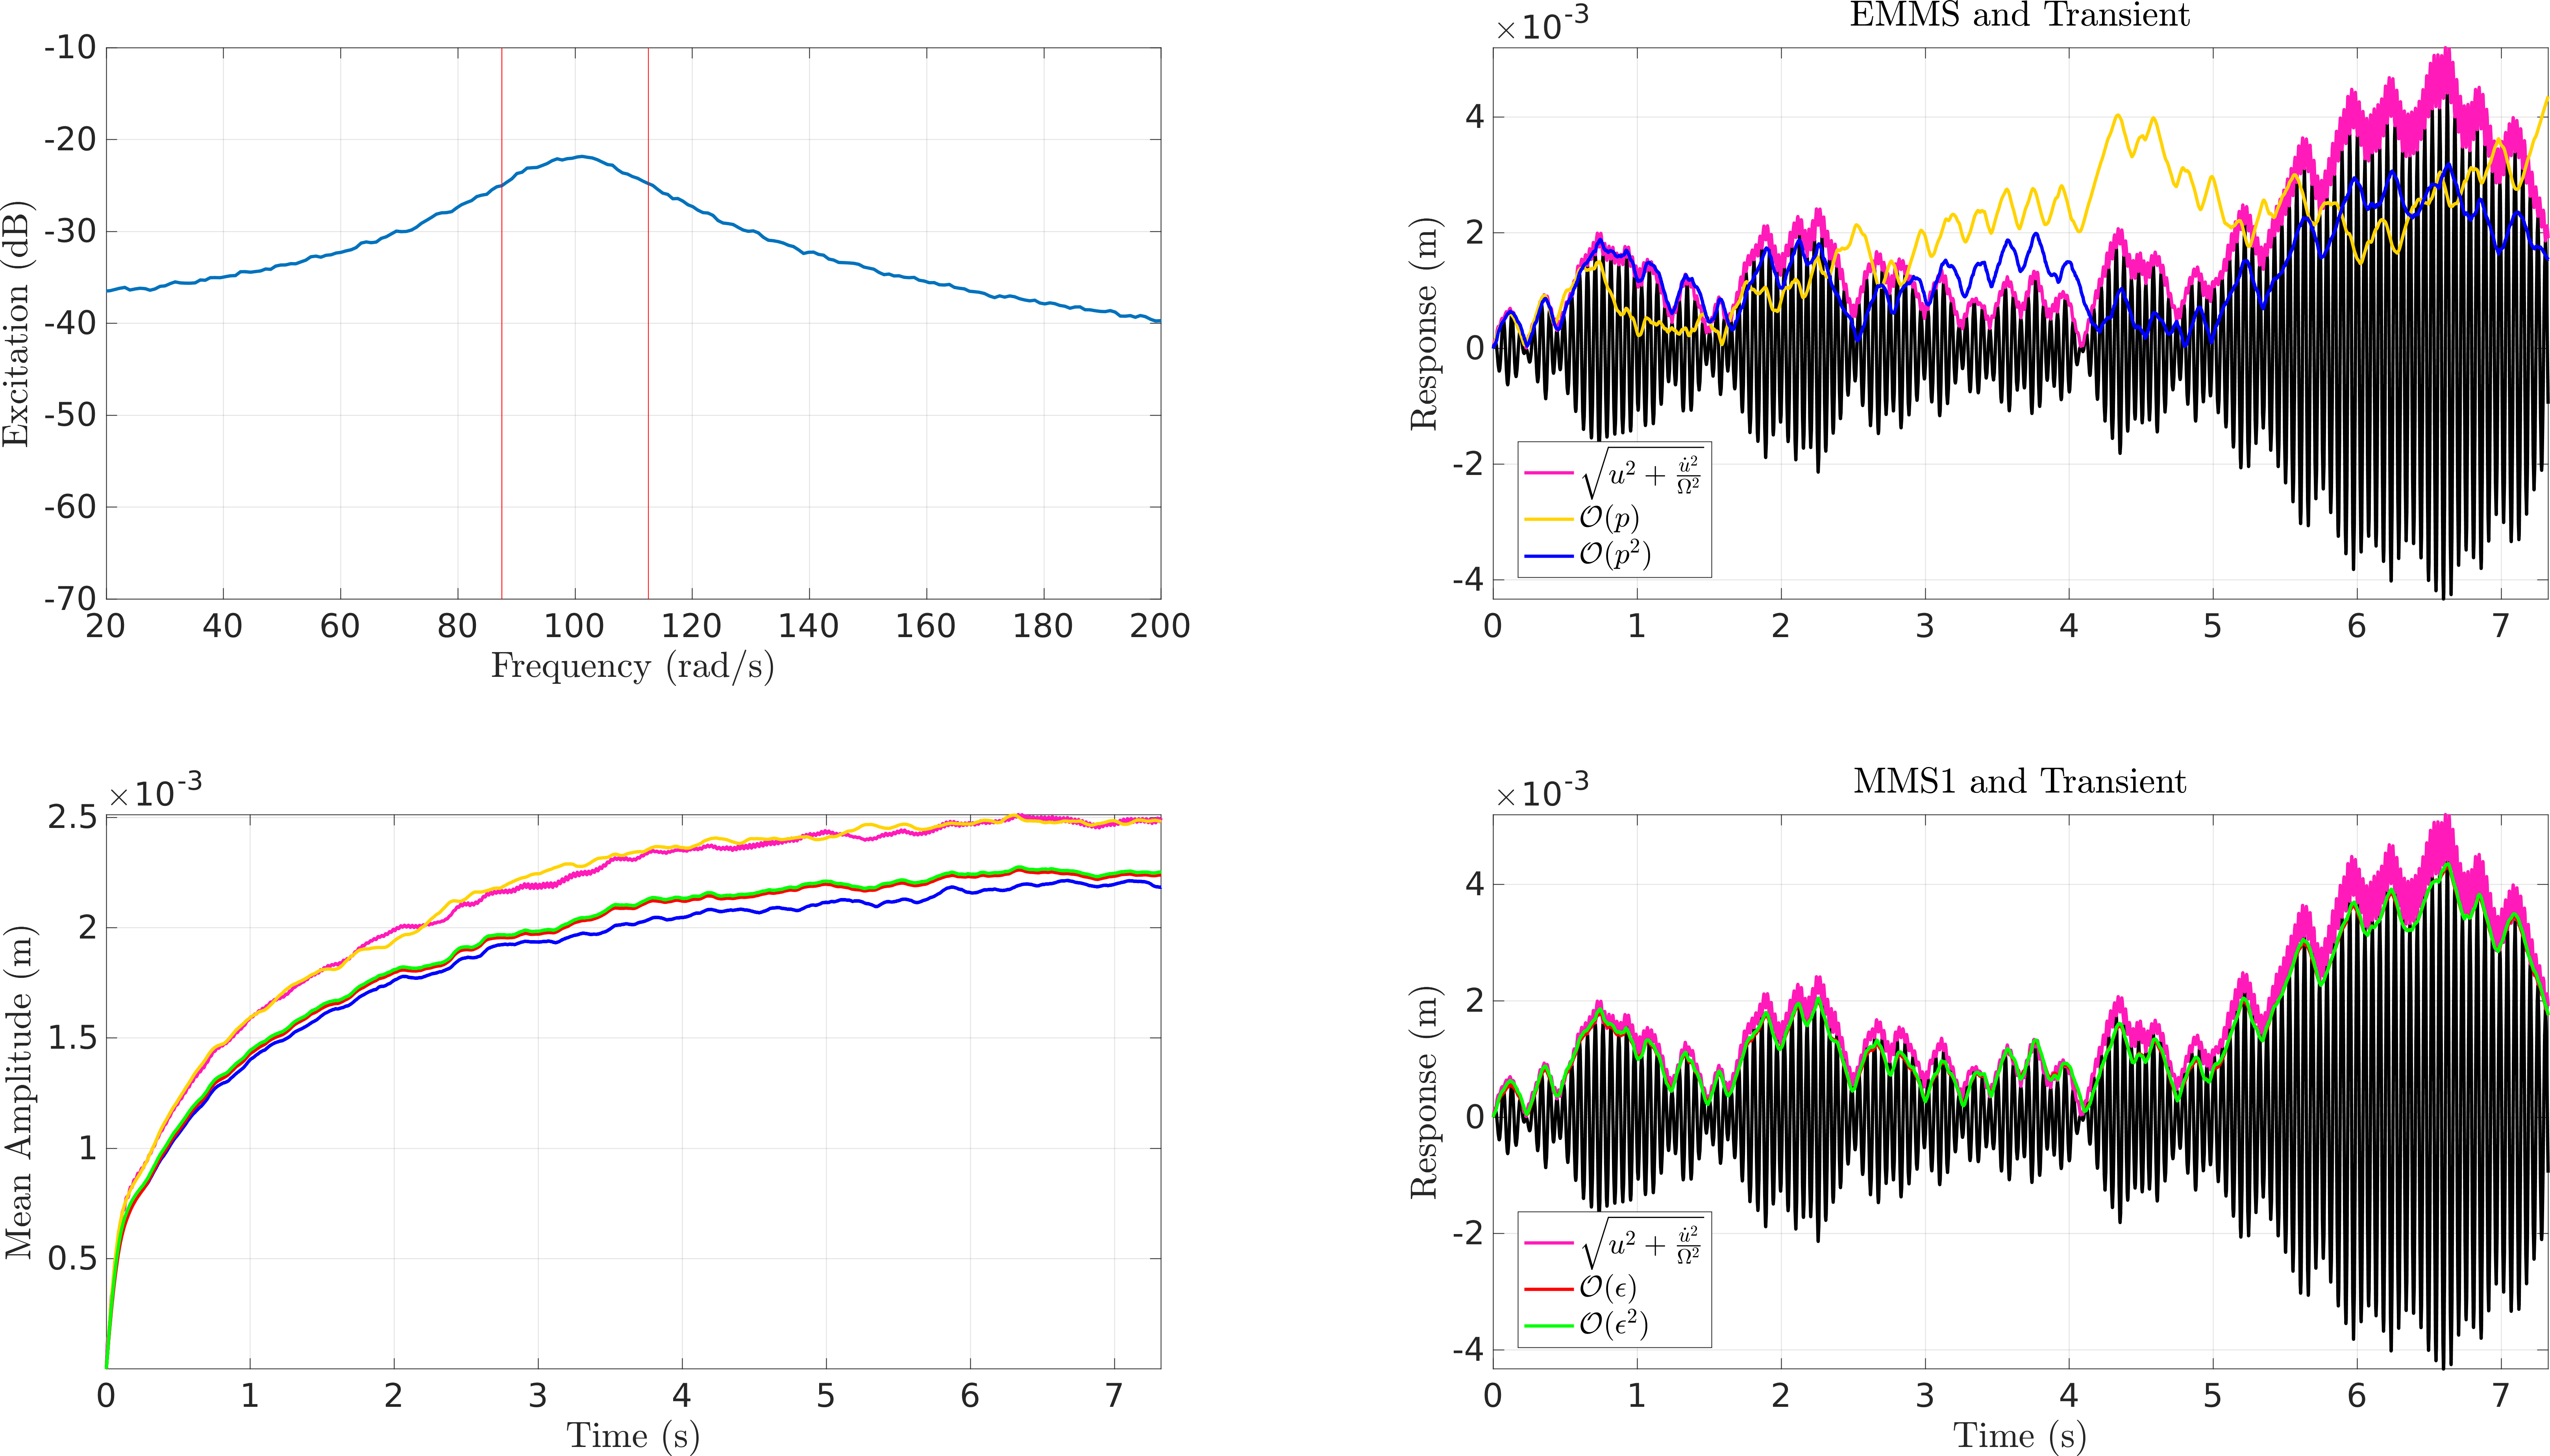
\includegraphics[width=.9\linewidth]{FIGS/C_linsystry0.png}
\caption{Slow-flow envelopes against the transient response}
\end{figure}
\end{figure}

\begin{figure}
\begin{figure}[htbp]
\centering
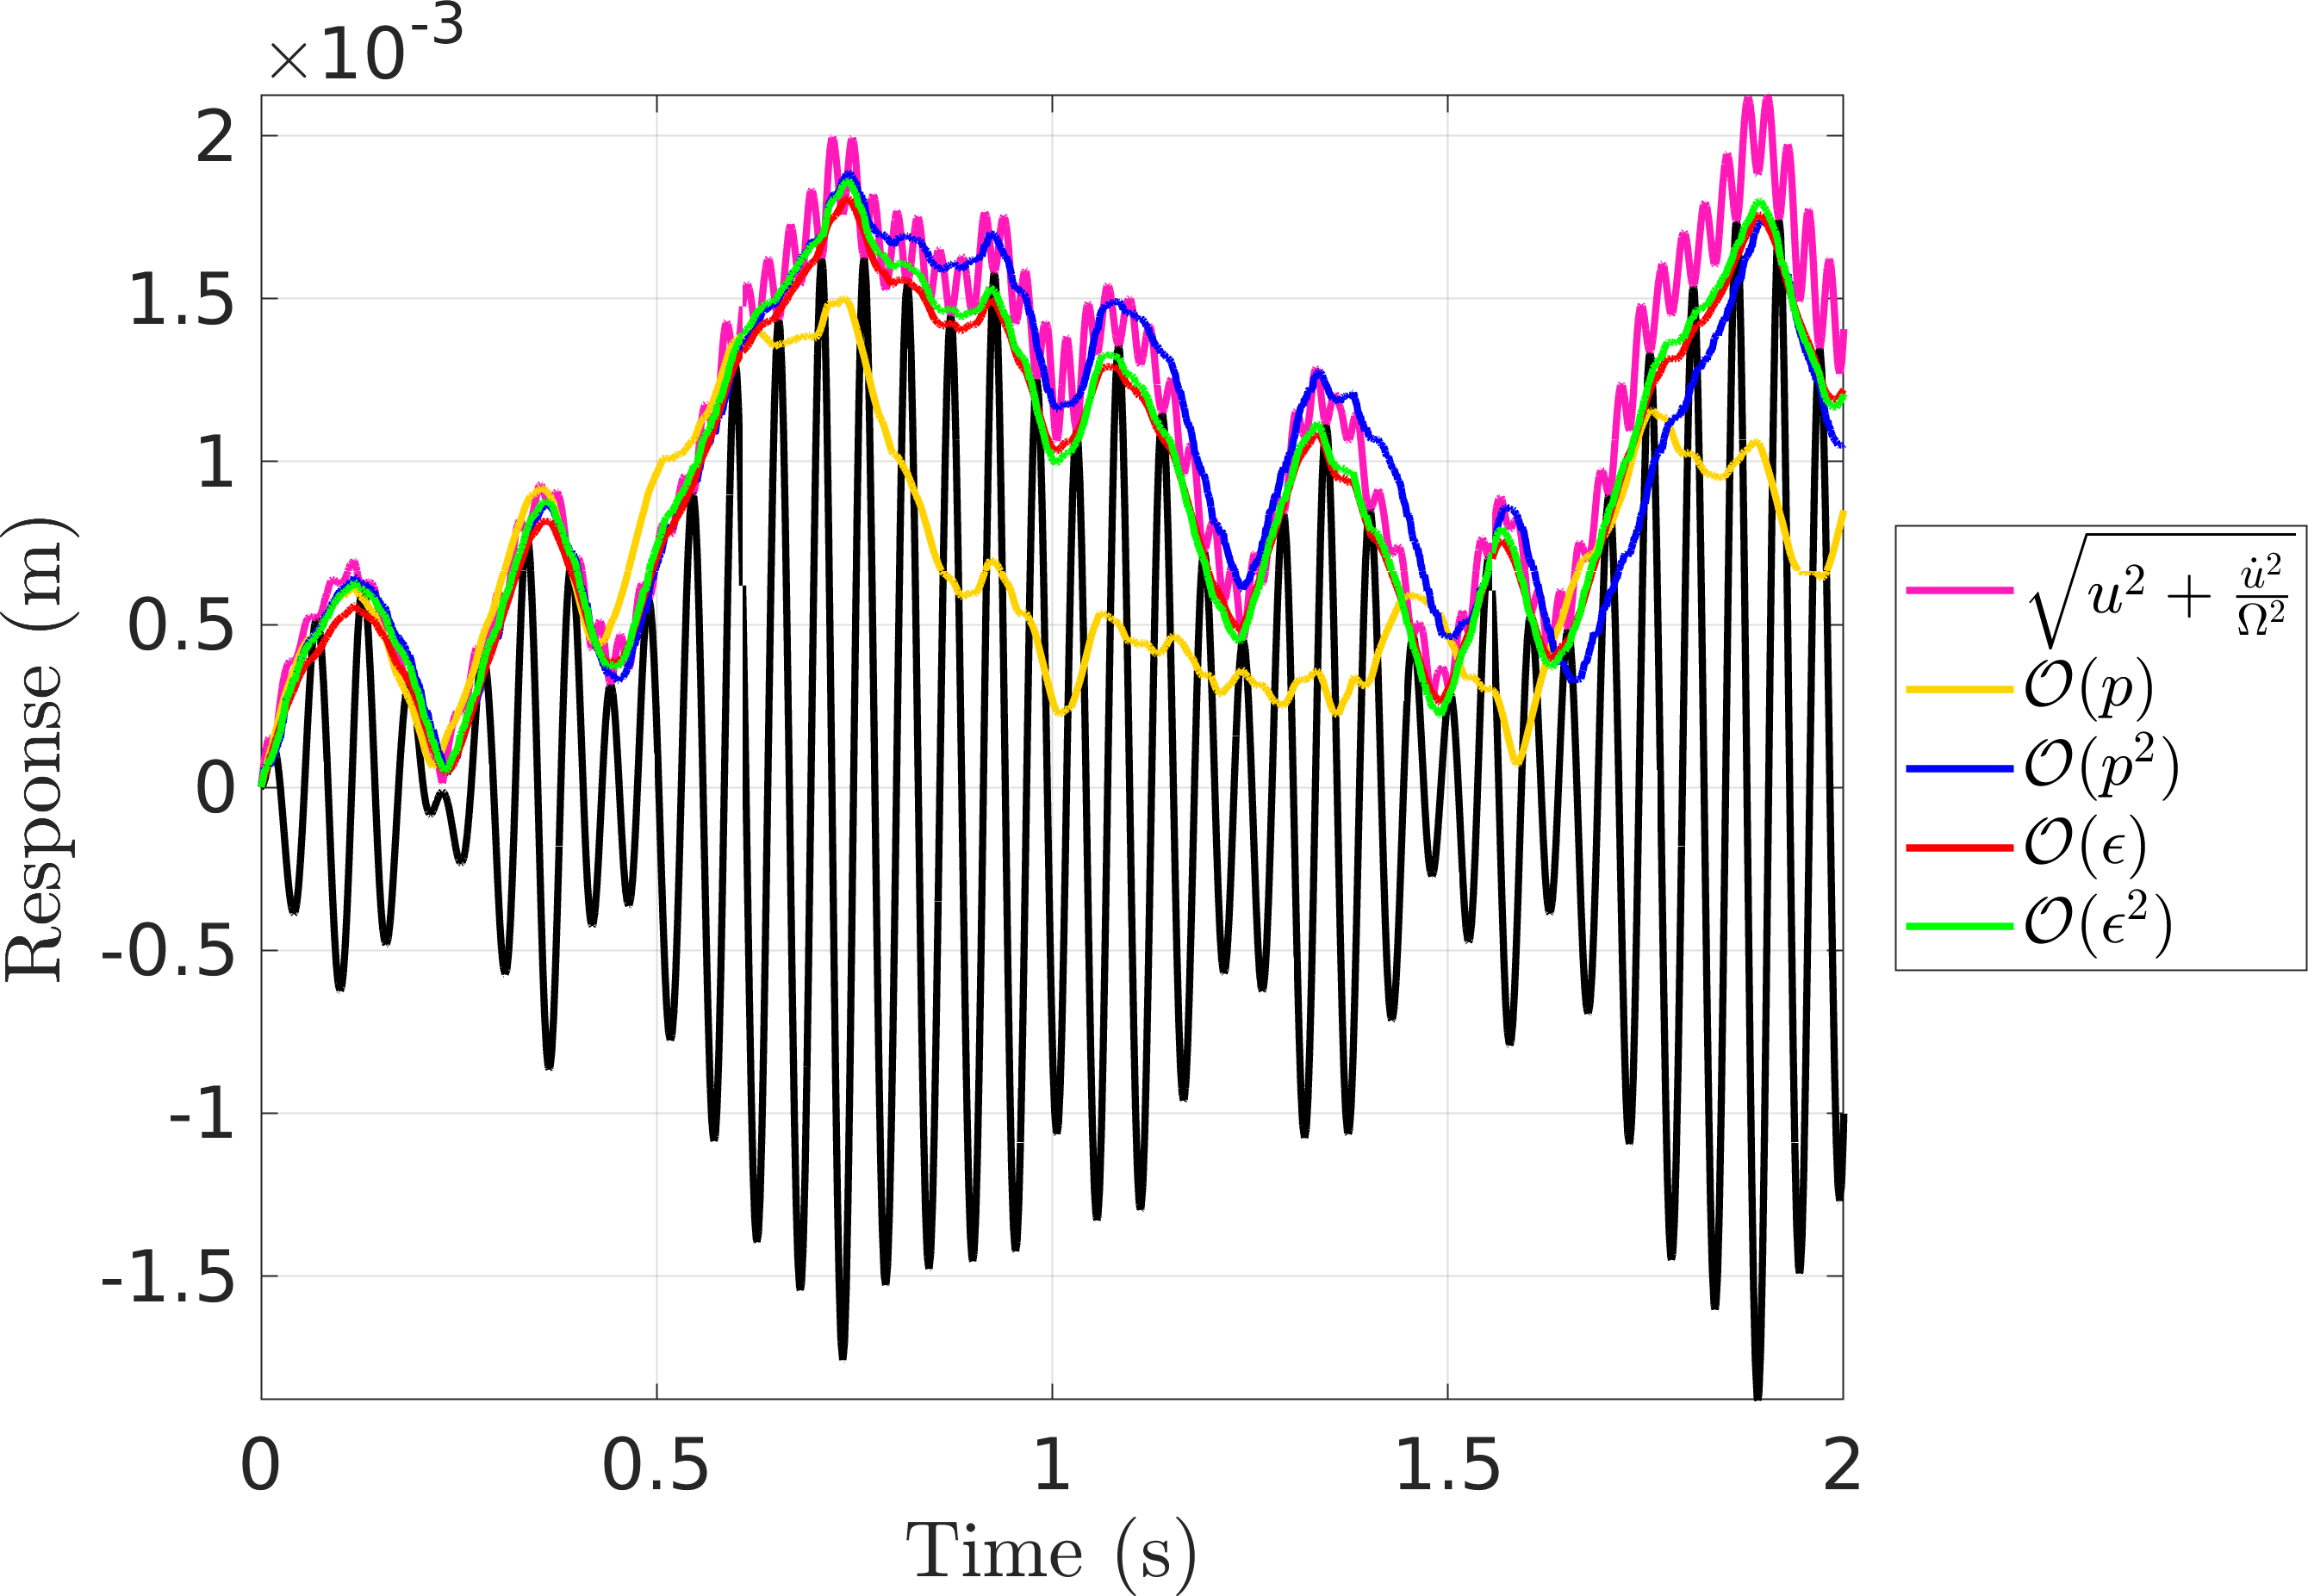
\includegraphics[width=.9\linewidth]{FIGS/C_ampzoomin.png}
\caption{A zoomed in view of the amplitude responses}
\end{figure}
\end{figure}
\item It can be seen that the CXA (\(\mathcal{O}(\textcolor{red}{\epsilon})\) EMMS) seems to match the \uline{\textbf{true amplitude mean}} much more closely than the others.
\item Looking closer seems to show that although the others track the true envelope closer, they seem to have some bias, while CXA does not. The MMS approaches, however, show better performance in standard deviation. 
\begin{figure}
\begin{figure}[htbp]
\centering
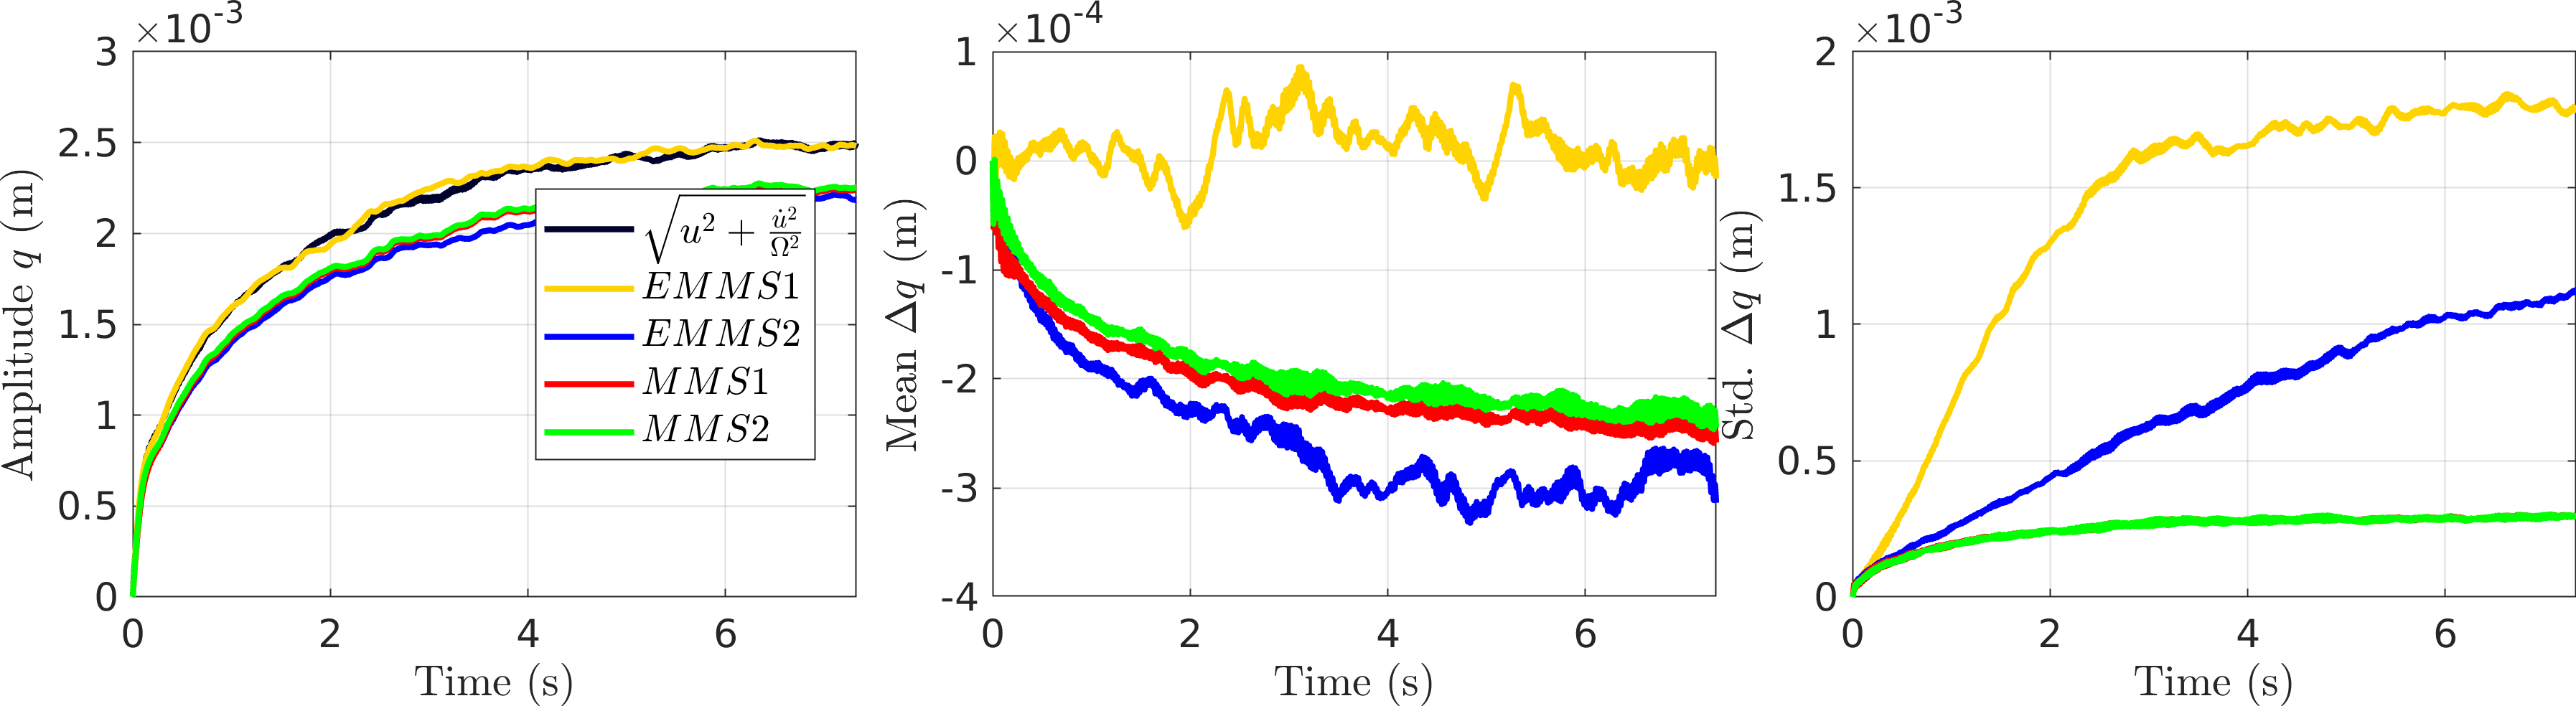
\includegraphics[width=.9\linewidth]{FIGS/C_invperf.png}
\caption{Performance of the different slow flow equations}
\end{figure}
\end{figure}
\begin{center}
\uline{\textbf{FPE Results}}
\end{center}
\item Here are the Eigenspectra of the FPK pencils. (Note that the analytical solution is written as \(p = \eta_i \phi_i e^{-\lambda_i t}\)). 
\begin{figure}[htbp]
\centering
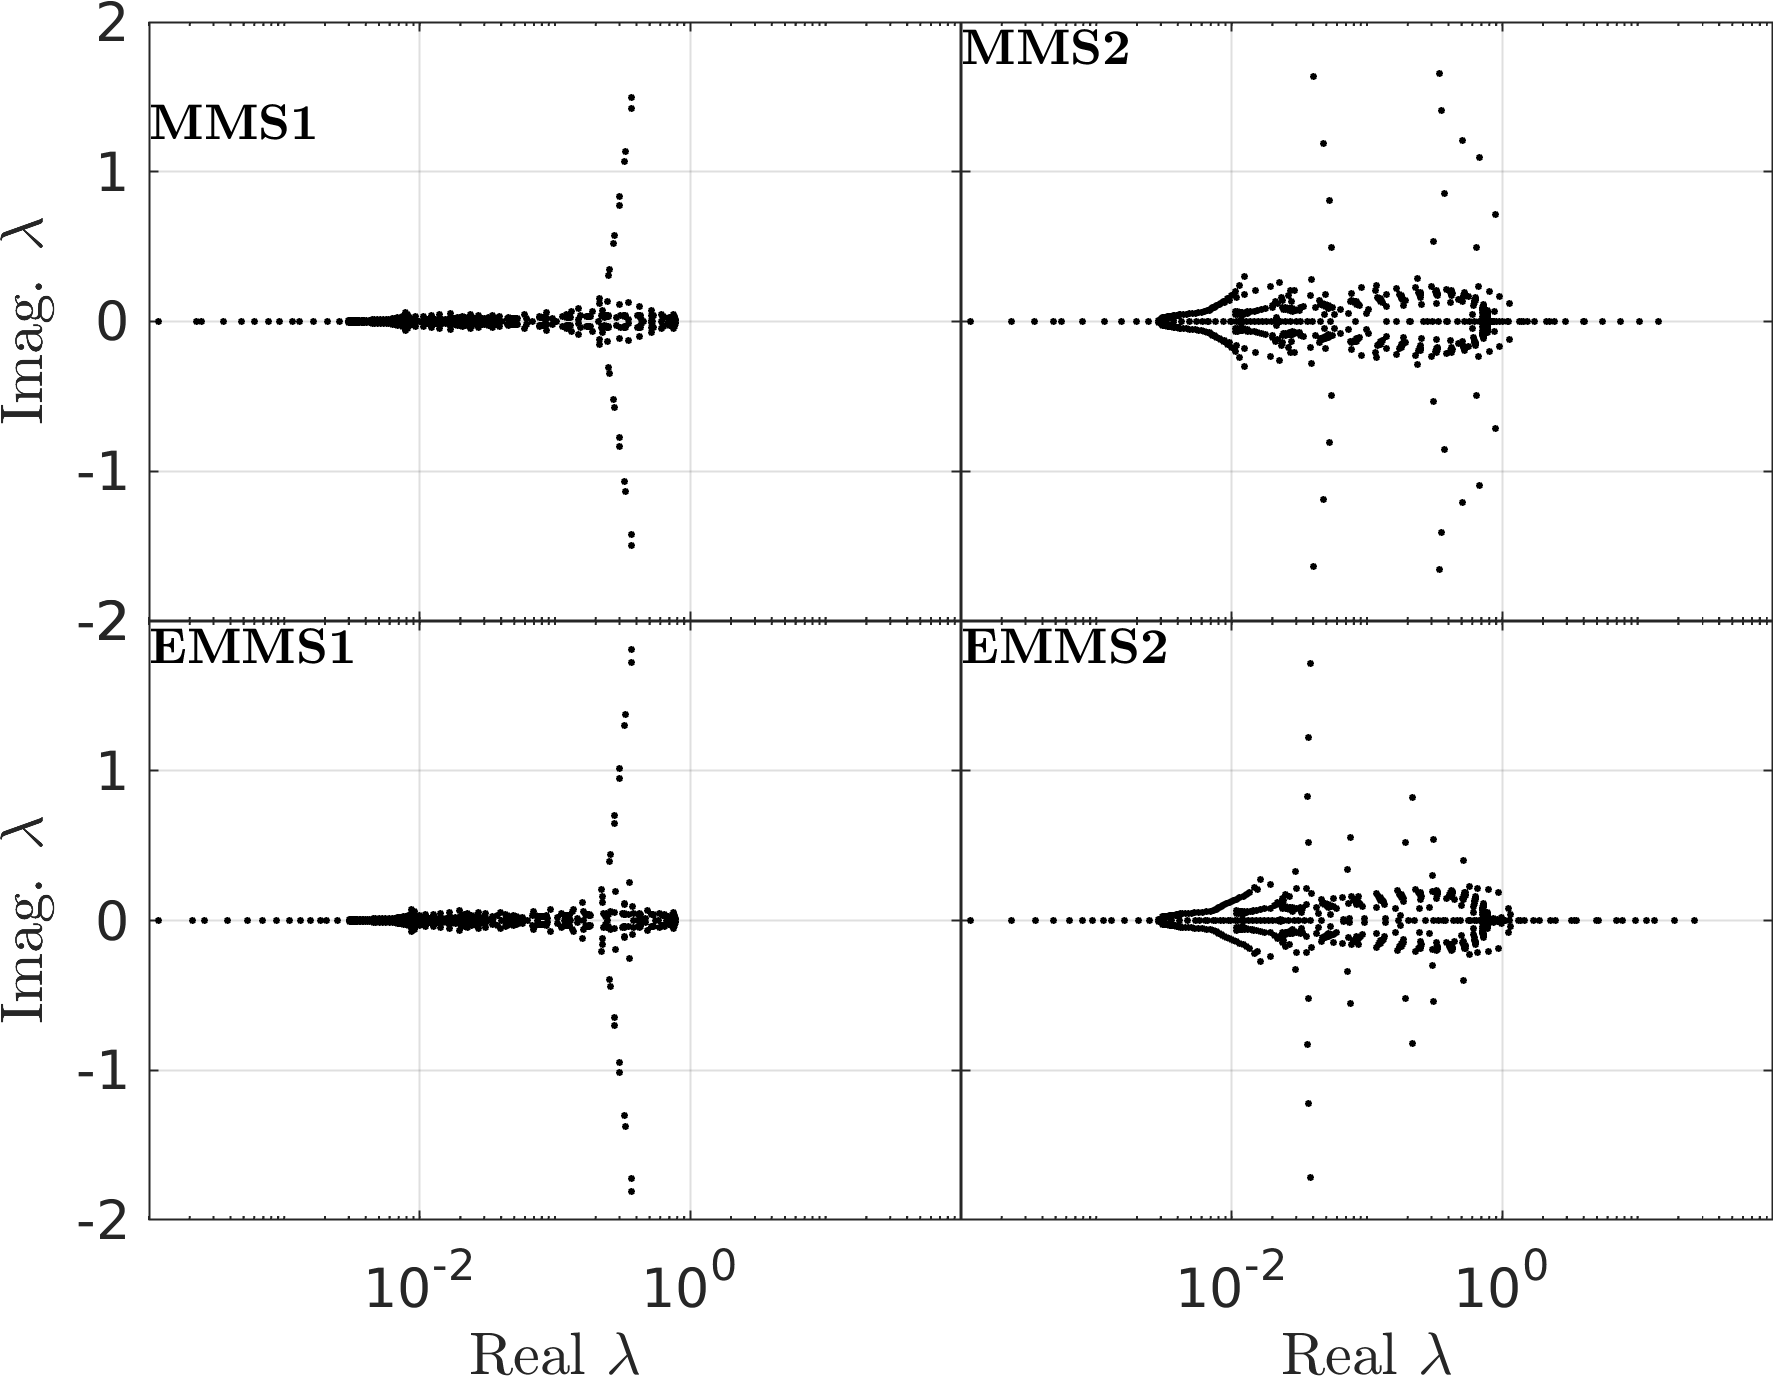
\includegraphics[width=.9\linewidth]{FIGS/F_EigSpec.png}
\caption{Eigenspectra of the FPK Pencils}
\end{figure}
\item In each case, the leading eigenvalue is numerically zero, indicating the existence of a steady-state.
\item The following are the PDFs computed using randomized transient simulations along with the PDF. The PDFs look to be \uline{\textbf{nominally similar}} for this case.
\item I haven't implemented a 2-parameter KS-test to be more rigorous, but this seems to be well-established and doable.
\end{itemize}
\begin{enumerate}
\item \(\mathcal{O}(\textcolor{red}{\epsilon})\) MMS
\label{sec:orgf90034b}
\item \(\mathcal{O}(\textcolor{red}{\epsilon^2})\) MMS
\label{sec:org90cc8cb}
\item CXA (\(\mathcal{O}(\textcolor{red}{p})\) EMMS)
\label{sec:org5ca6449}
\item \(\mathcal{O}(\textcolor{red}{p^2})\) EMMS
\label{sec:orgbf75961}
\end{enumerate}
\subsection{Questions on Path Forward}
\label{sec:org8e63d98}
\begin{itemize}
\item We now have the capability of repeating this analysis for any system whose nonlinear modal characteristics are known.
\item I have planned to use \uline{\textbf{EPMC results from the RuBber Beam}} to generate nonlinear results.
\item Any specific cases I should focus on?
\item We could have an \uline{\textbf{experimental campaign}} focused on
\begin{itemize}
\item Obtaining backbones with PLL -> FPE pdf predictions
\item Conducting phase-noise excitation and validating
\item The same backbones could also be used for quasi-periodic synthesis.
\end{itemize}
\end{itemize}
\subsubsection{Something that caught my eye: "Stochastic jump" phenomena \citeprocitem{4}{[4]}}
\label{sec:org831f6aa}
\subsection{Meeting Notes}
\label{sec:org7afa7b7}
\begin{enumerate}
\item Cases with co-existing stable solutions are certainly more interesting.
\begin{itemize}
\item Doing an example with a reasonably soft impact might be interesting.
\end{itemize}
\item What are the kinds of analysis we can do once we have the density distribution?
\begin{itemize}
\item For multi-valued response regimes, we could compute transition likelihoods.
\end{itemize}
\item We should move on to multi-input cases, where there is \textbf{spatially correlated} random input.
\begin{itemize}
\item Maybe we can model these as \(\frac{F_1}{2}e^{i\sigma_1}+\frac{F_2}{2}e^{i\sigma_2}+\dots\) ?
\item Using the FPE in this context really has lots of relevance since doing Monte-Carlo here is quite infeasible due to the potentially large number of independent random variables.
\item The \textbf{vortex-induced cable vibration problem} that Tobi worked on presents such a case. Could be interesting to have a look at how the excitation is modeled.
\end{itemize}
\item It is important that the example we choose shows that we NEED to model it is a non-linear system (statistical linearization would lead to spurious results). This would really drive home the point of the necessity of this formulation.
\begin{itemize}
\item An added aspect is that using NMA backbones allow us to use it for MDOF problems, where, already, computational savings are possible.
\end{itemize}
\end{enumerate}

\section{Week 2}
\label{sec:org0173fe1}
\subsection{Validation on Nonlinear Systems}
\label{sec:org8115394}
\begin{itemize}
\item The implementation for the most general case with support for nonlinear MDOF oscillators specified through \(\omega_0(q), \zeta(q), \psi(q)\) is complete.
\item I only have results for an SDOF oscillator here, more soon.
\item The dependencies of the second order formulae on the different terms are tabulated below:
\begin{center}
\begin{tabular}{llllllllll}
Formula & \(\omega\quad\) & \(\zeta\quad\) & \(\psi\quad\) & \(\omega'\quad\) & \(\zeta'\quad\) & \(\psi'\quad\) & \(\omega''\quad\) & \(\zeta''\quad\) & \(\psi''\quad\)\\[0pt]
\hline
\(\mathcal{O}(\textcolor{red}{\epsilon})\) MMS & \(\checkmark\) & \(\checkmark\) & \(\checkmark\) & \(\checkmark\) &  &  &  &  & \\[0pt]
\(\mathcal{O}(\textcolor{red}{\epsilon^2})\) MMS & \(\checkmark\) & \(\checkmark\) & \(\checkmark\) & \(\checkmark\) & \(\checkmark\) & \(\checkmark\) & \(\checkmark\) &  & \\[0pt]
\(\mathcal{O}(\textcolor{red}{p})\) EMMS & \(\checkmark\) & \(\checkmark\) & \(\checkmark\) &  &  &  &  &  & \\[0pt]
\(\mathcal{O}(\textcolor{red}{p^2})\) MMS & \(\checkmark\) & \(\checkmark\) & \(\checkmark\) & \(\checkmark\) & \(\checkmark\) & \(\checkmark\) &  &  & \\[0pt]
\end{tabular}
\end{center}
\end{itemize}
\subsubsection{SDOF Duffing Oscillator}
\label{sec:org9b10f29}
\begin{itemize}
\item Considered EOM:
$$ \ddot{x} + 2\zeta_n\omega_n \dot{x}+\omega_n^2x + \alpha x^3=F\cos\sigma, $$
with parameters,
$$ \omega_0=1\,rad/s,\quad \zeta_n=10^{-3},\quad \alpha=0.2,\quad F=0.07\,N. $$
\item Used EPMC to compute the backbones first
\begin{figure}
\begin{figure}[htbp]
\centering
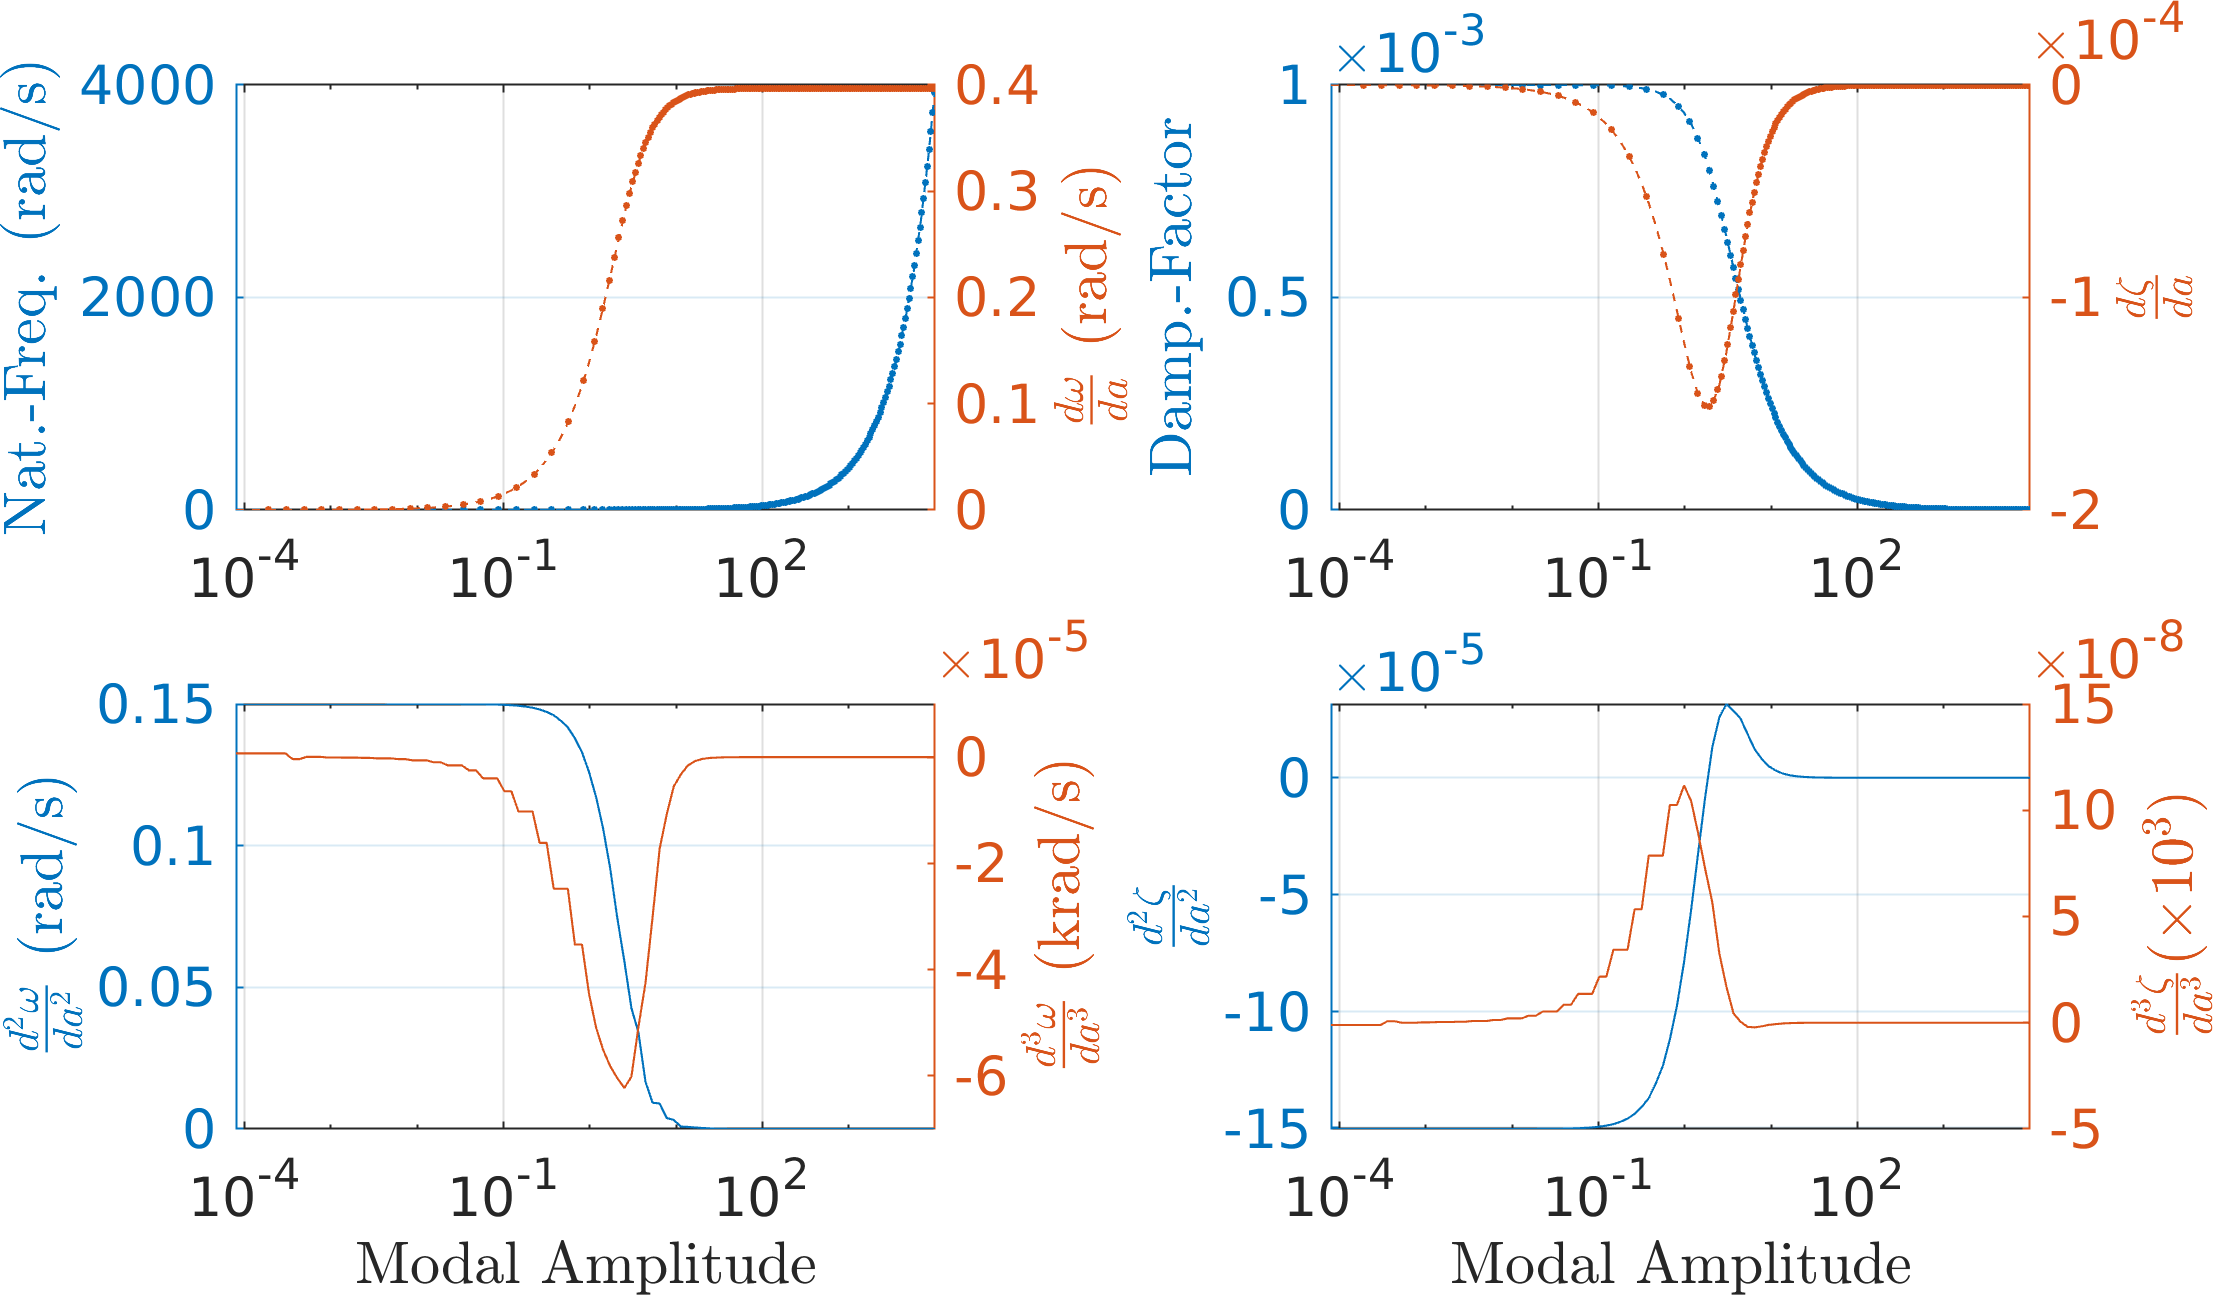
\includegraphics[width=.9\linewidth]{FIGS/G1_SDOFEPMC_duffing.png}
\caption{EPMC Backbone for the SDOF Duffing oscillator}
\end{figure}
\end{figure}
\item This is next used to obtain the PDF of the slow flow system using the four different formulations. Here is a summary.
\item It looks like CXA (\(\mathcal{O}(\textcolor{red}{p})\) EMMS) seems to underpredict the density of the higher amplitude.
\end{itemize}
\begin{enumerate}
\item \(\mathcal{O}(\textcolor{red}{\epsilon})\) MMS
\label{sec:orgcc35ec9}
\begin{figure}
\begin{figure}[htbp]
\centering
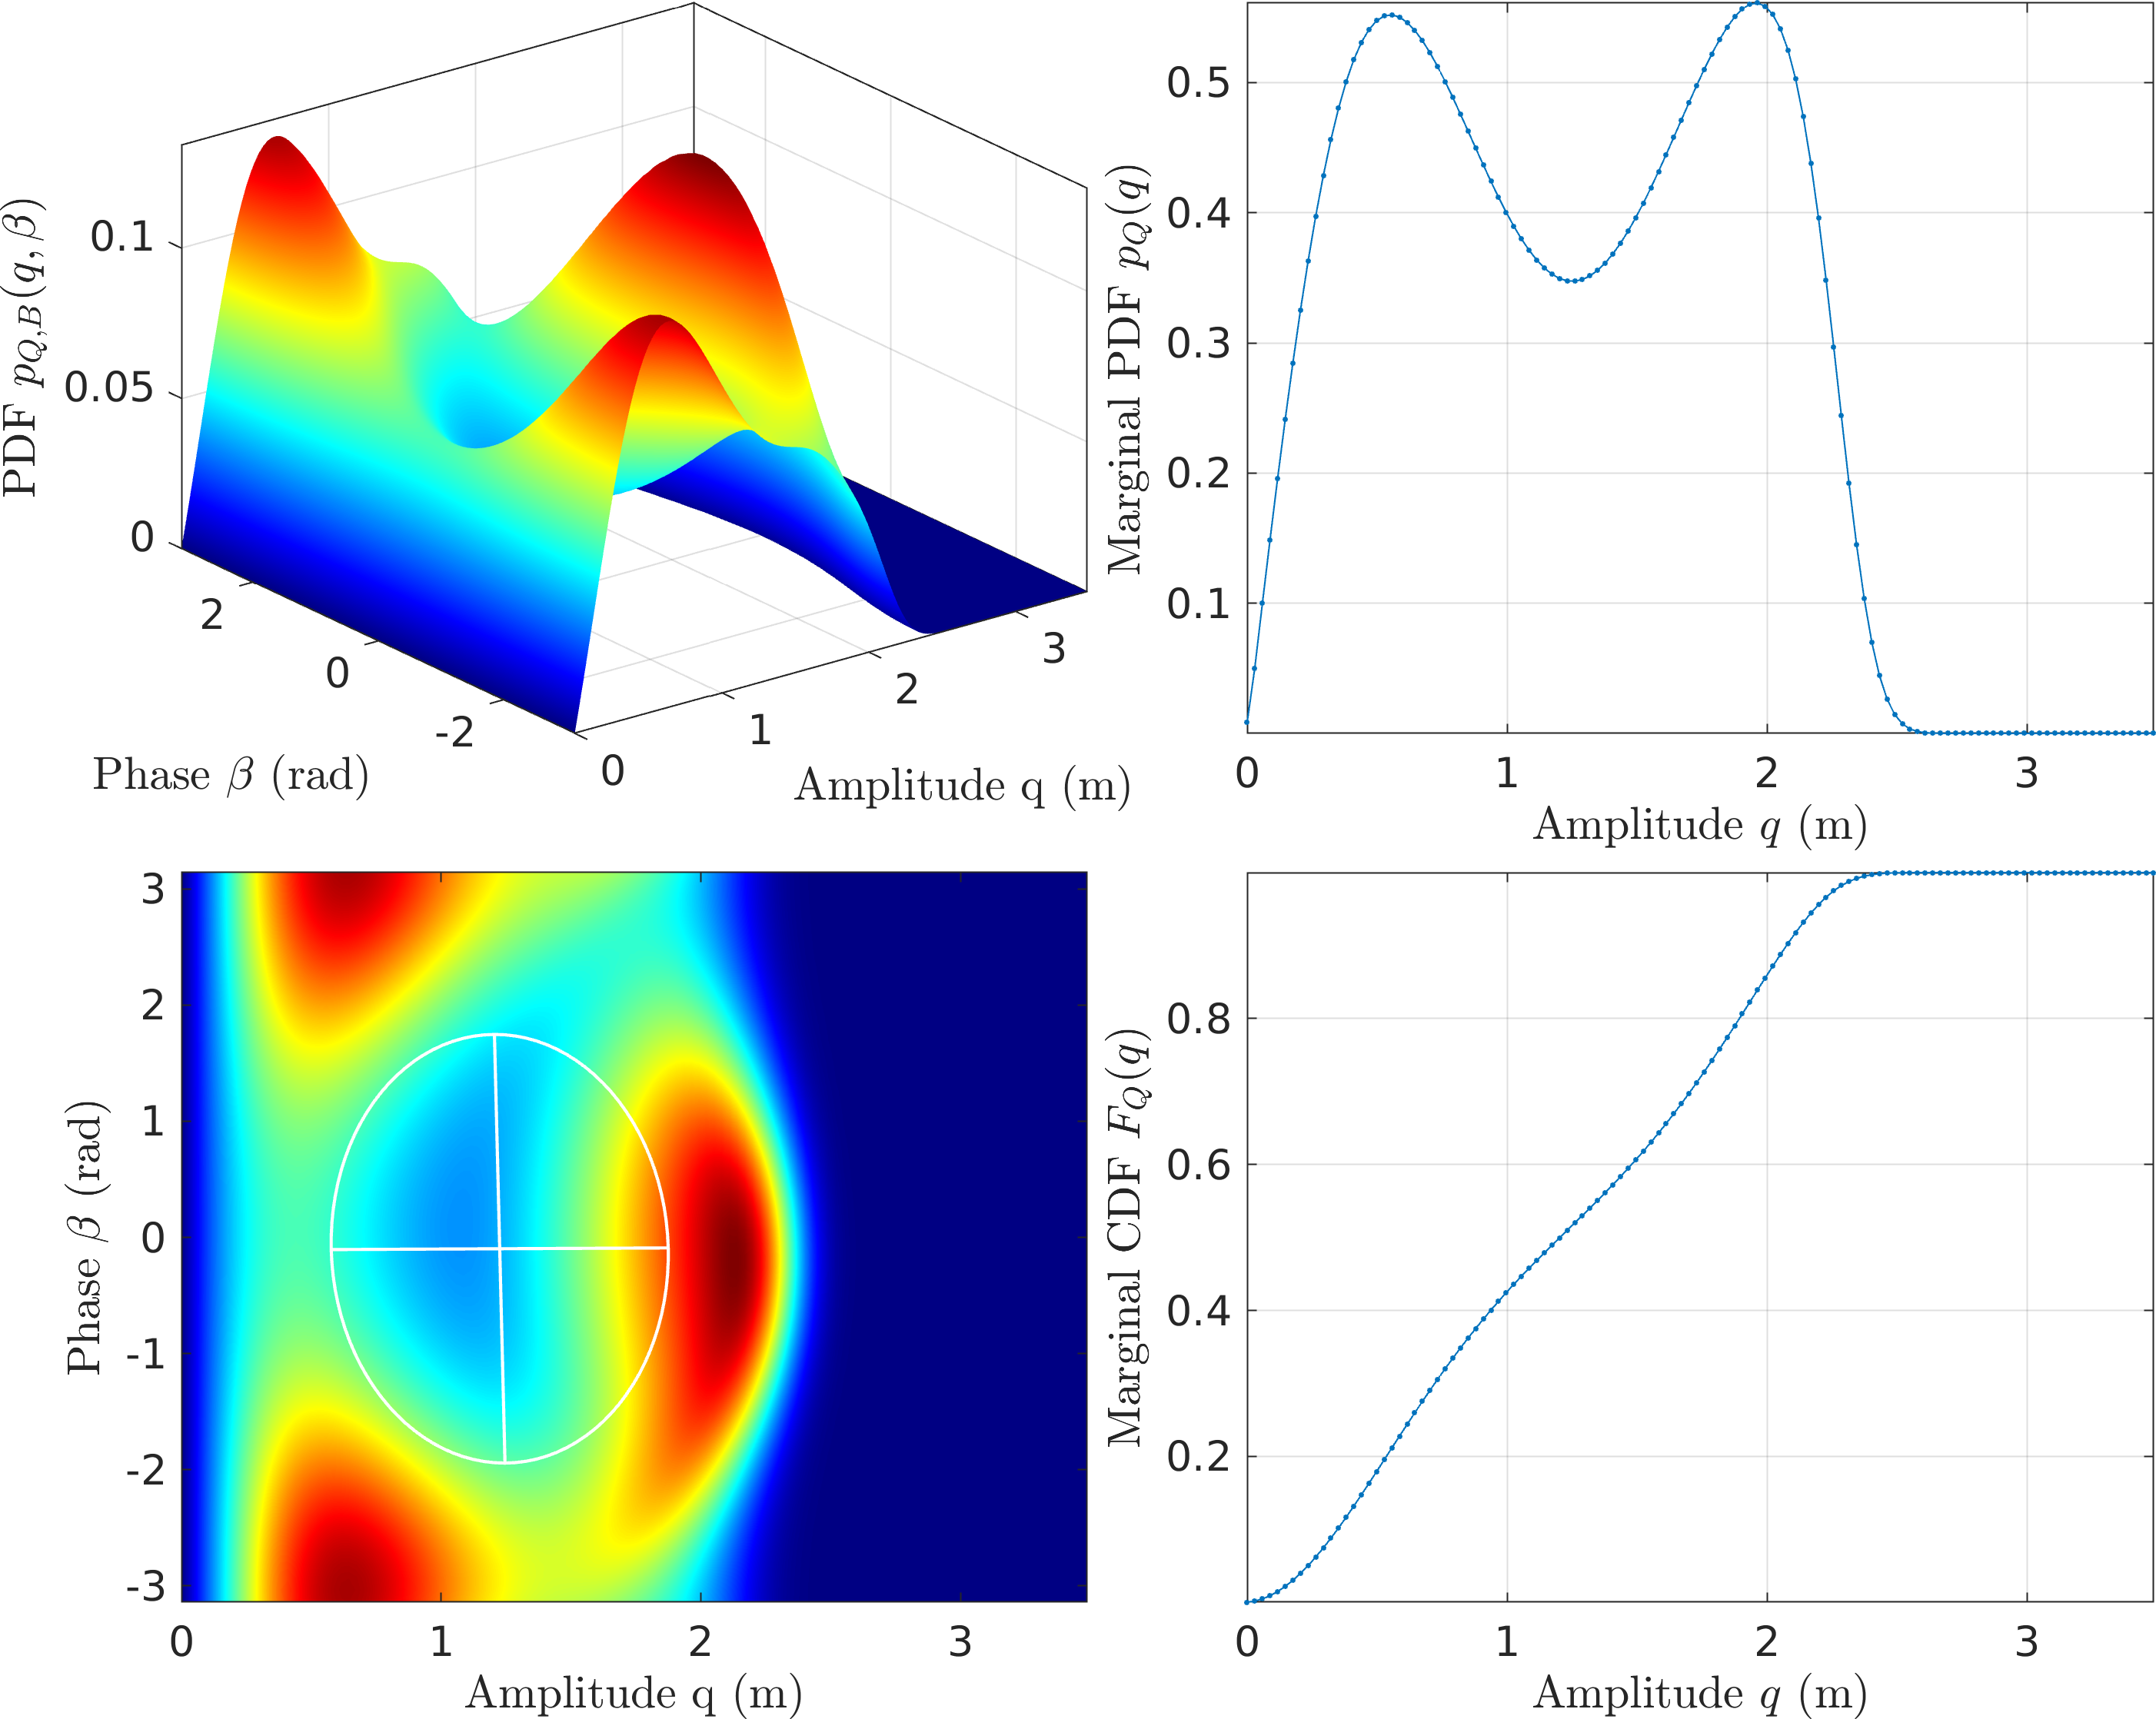
\includegraphics[width=.9\linewidth]{FIGS/G3_SDOFFPE_duffing_mms1.png}
\caption{FPE Results for the Duffing Oscillator with MMS1}
\end{figure}
\end{figure}
\item \(\mathcal{O}(\textcolor{red}{\epsilon^2})\) MMS
\label{sec:orgef43544}
\begin{figure}
\begin{figure}[htbp]
\centering
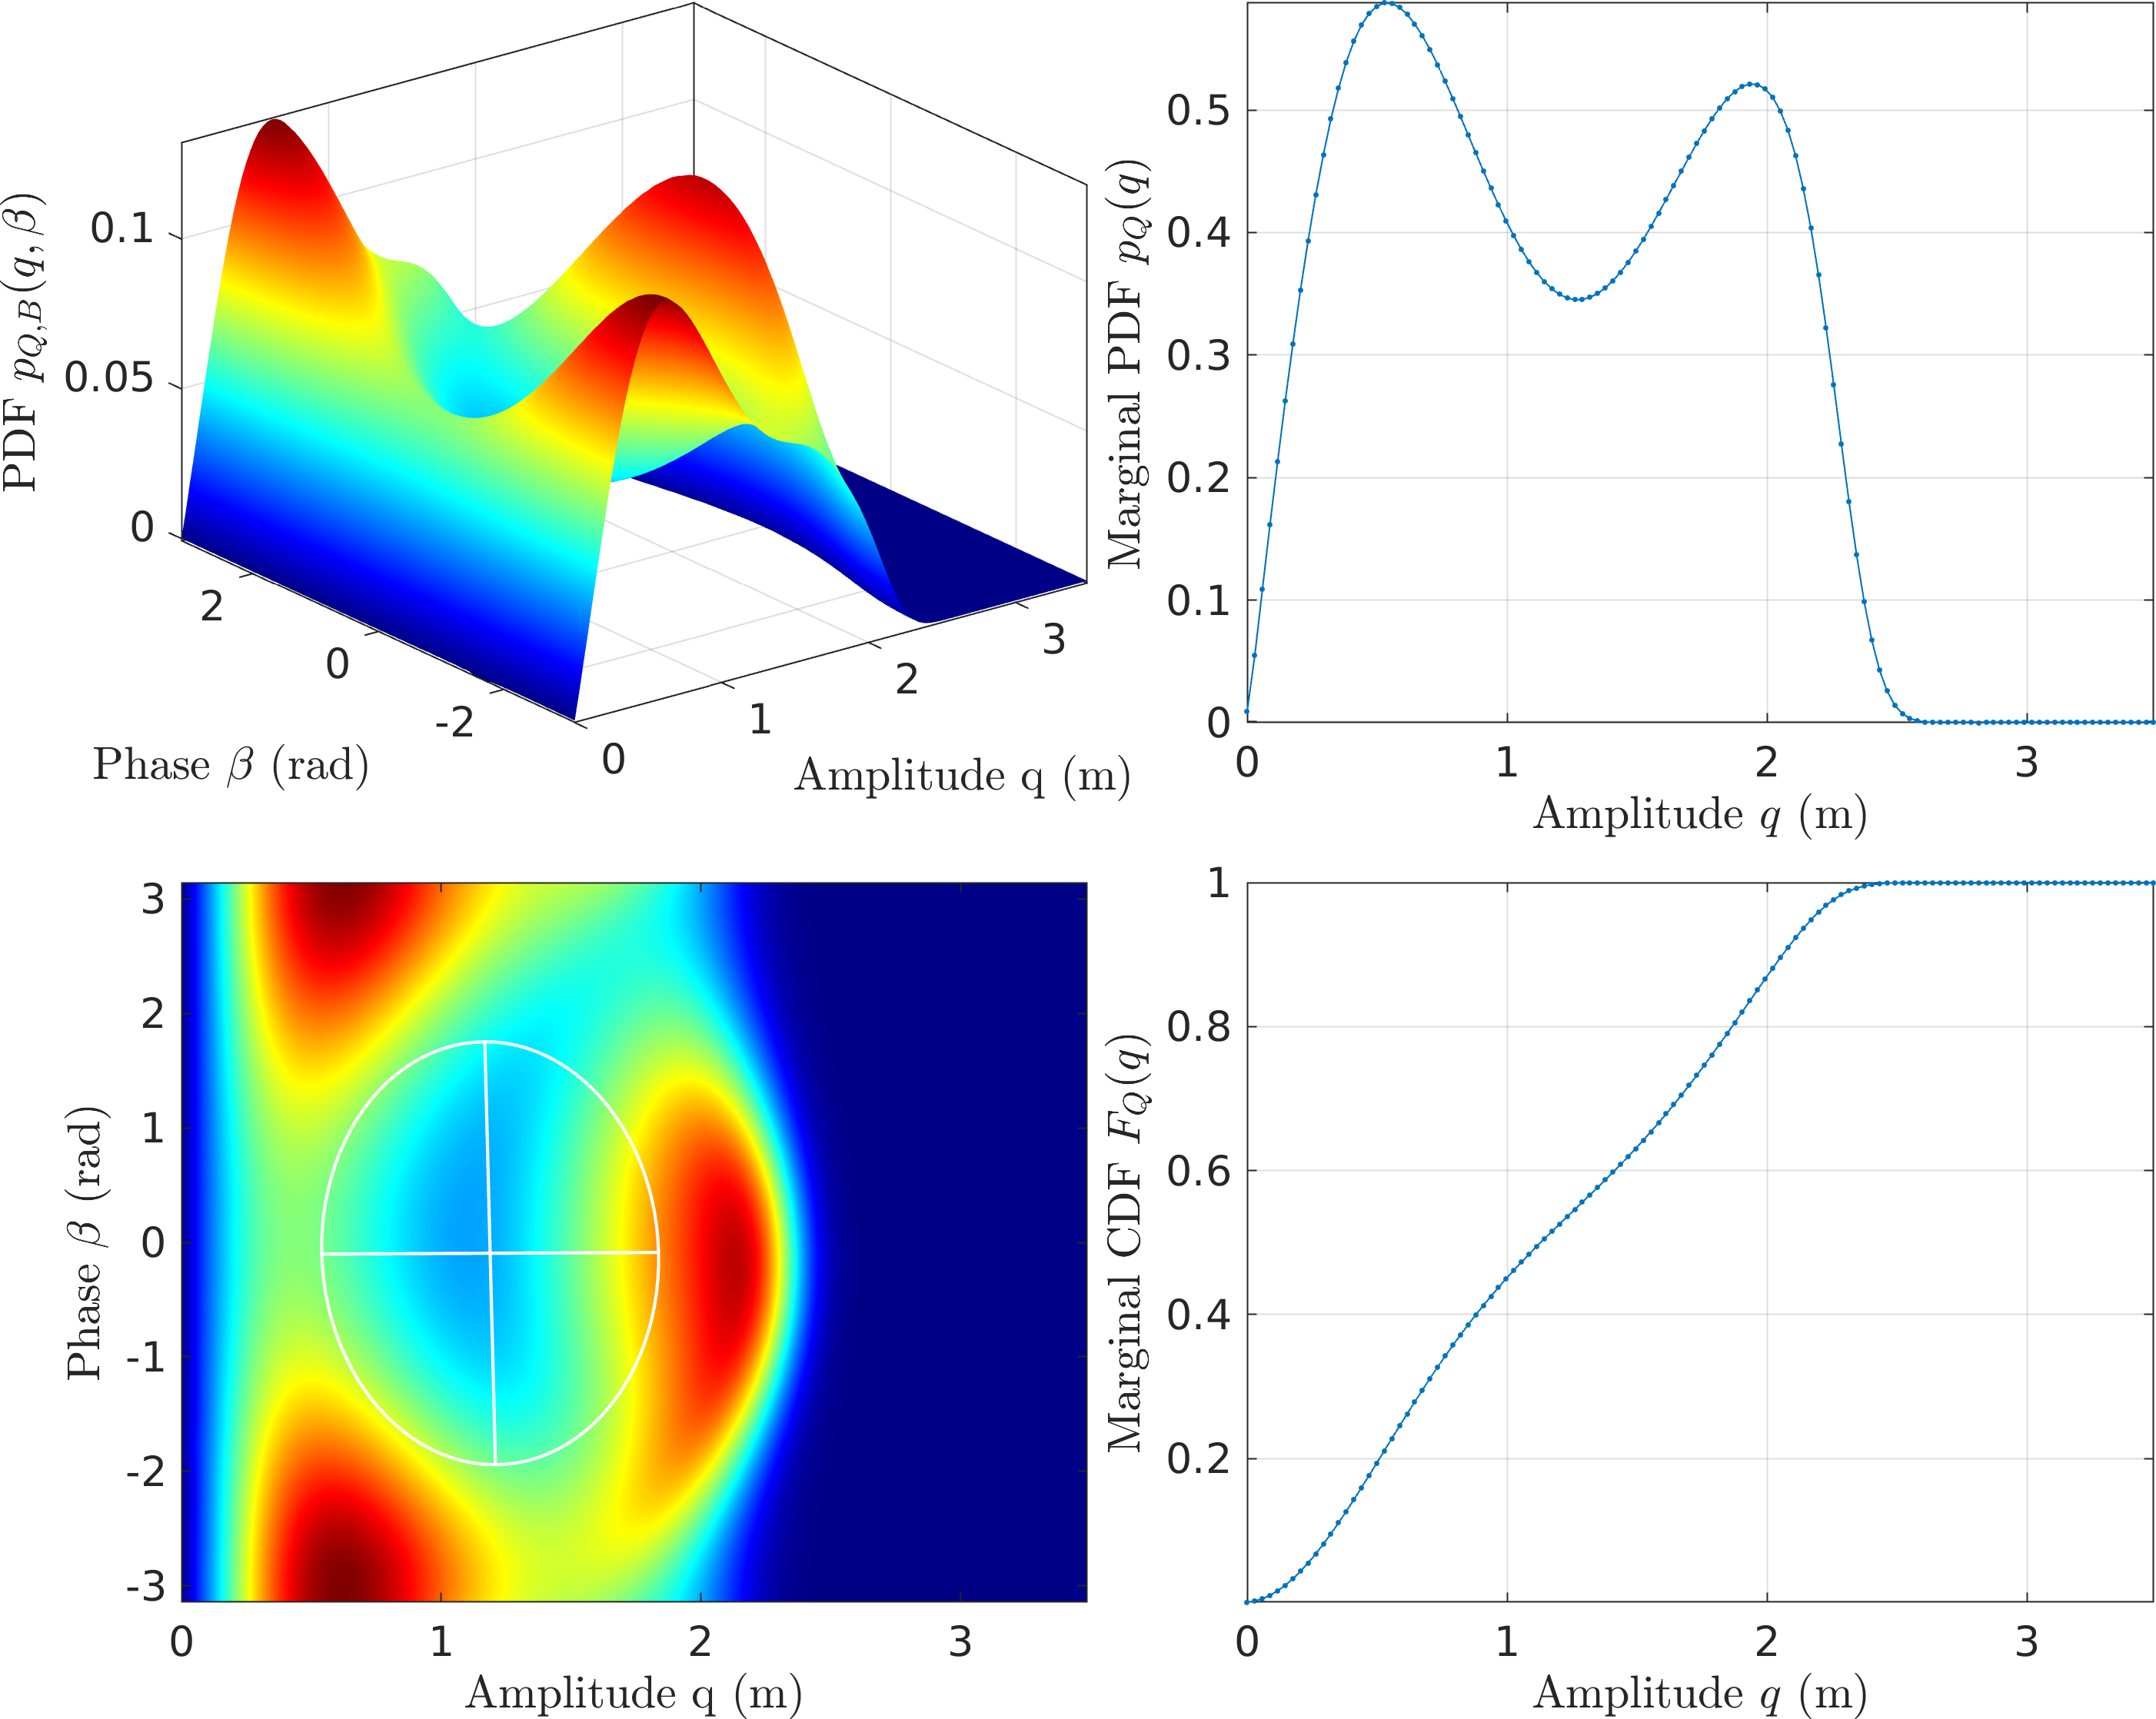
\includegraphics[width=.9\linewidth]{FIGS/G3_SDOFFPE_duffing_mms2.png}
\caption{FPE Results for the Duffing Oscillator with MMS2}
\end{figure}
\end{figure}
\item CXA (\(\mathcal{O}(\textcolor{red}{p})\) EMMS)
\label{sec:org1a8606c}
\begin{figure}
\begin{figure}[htbp]
\centering
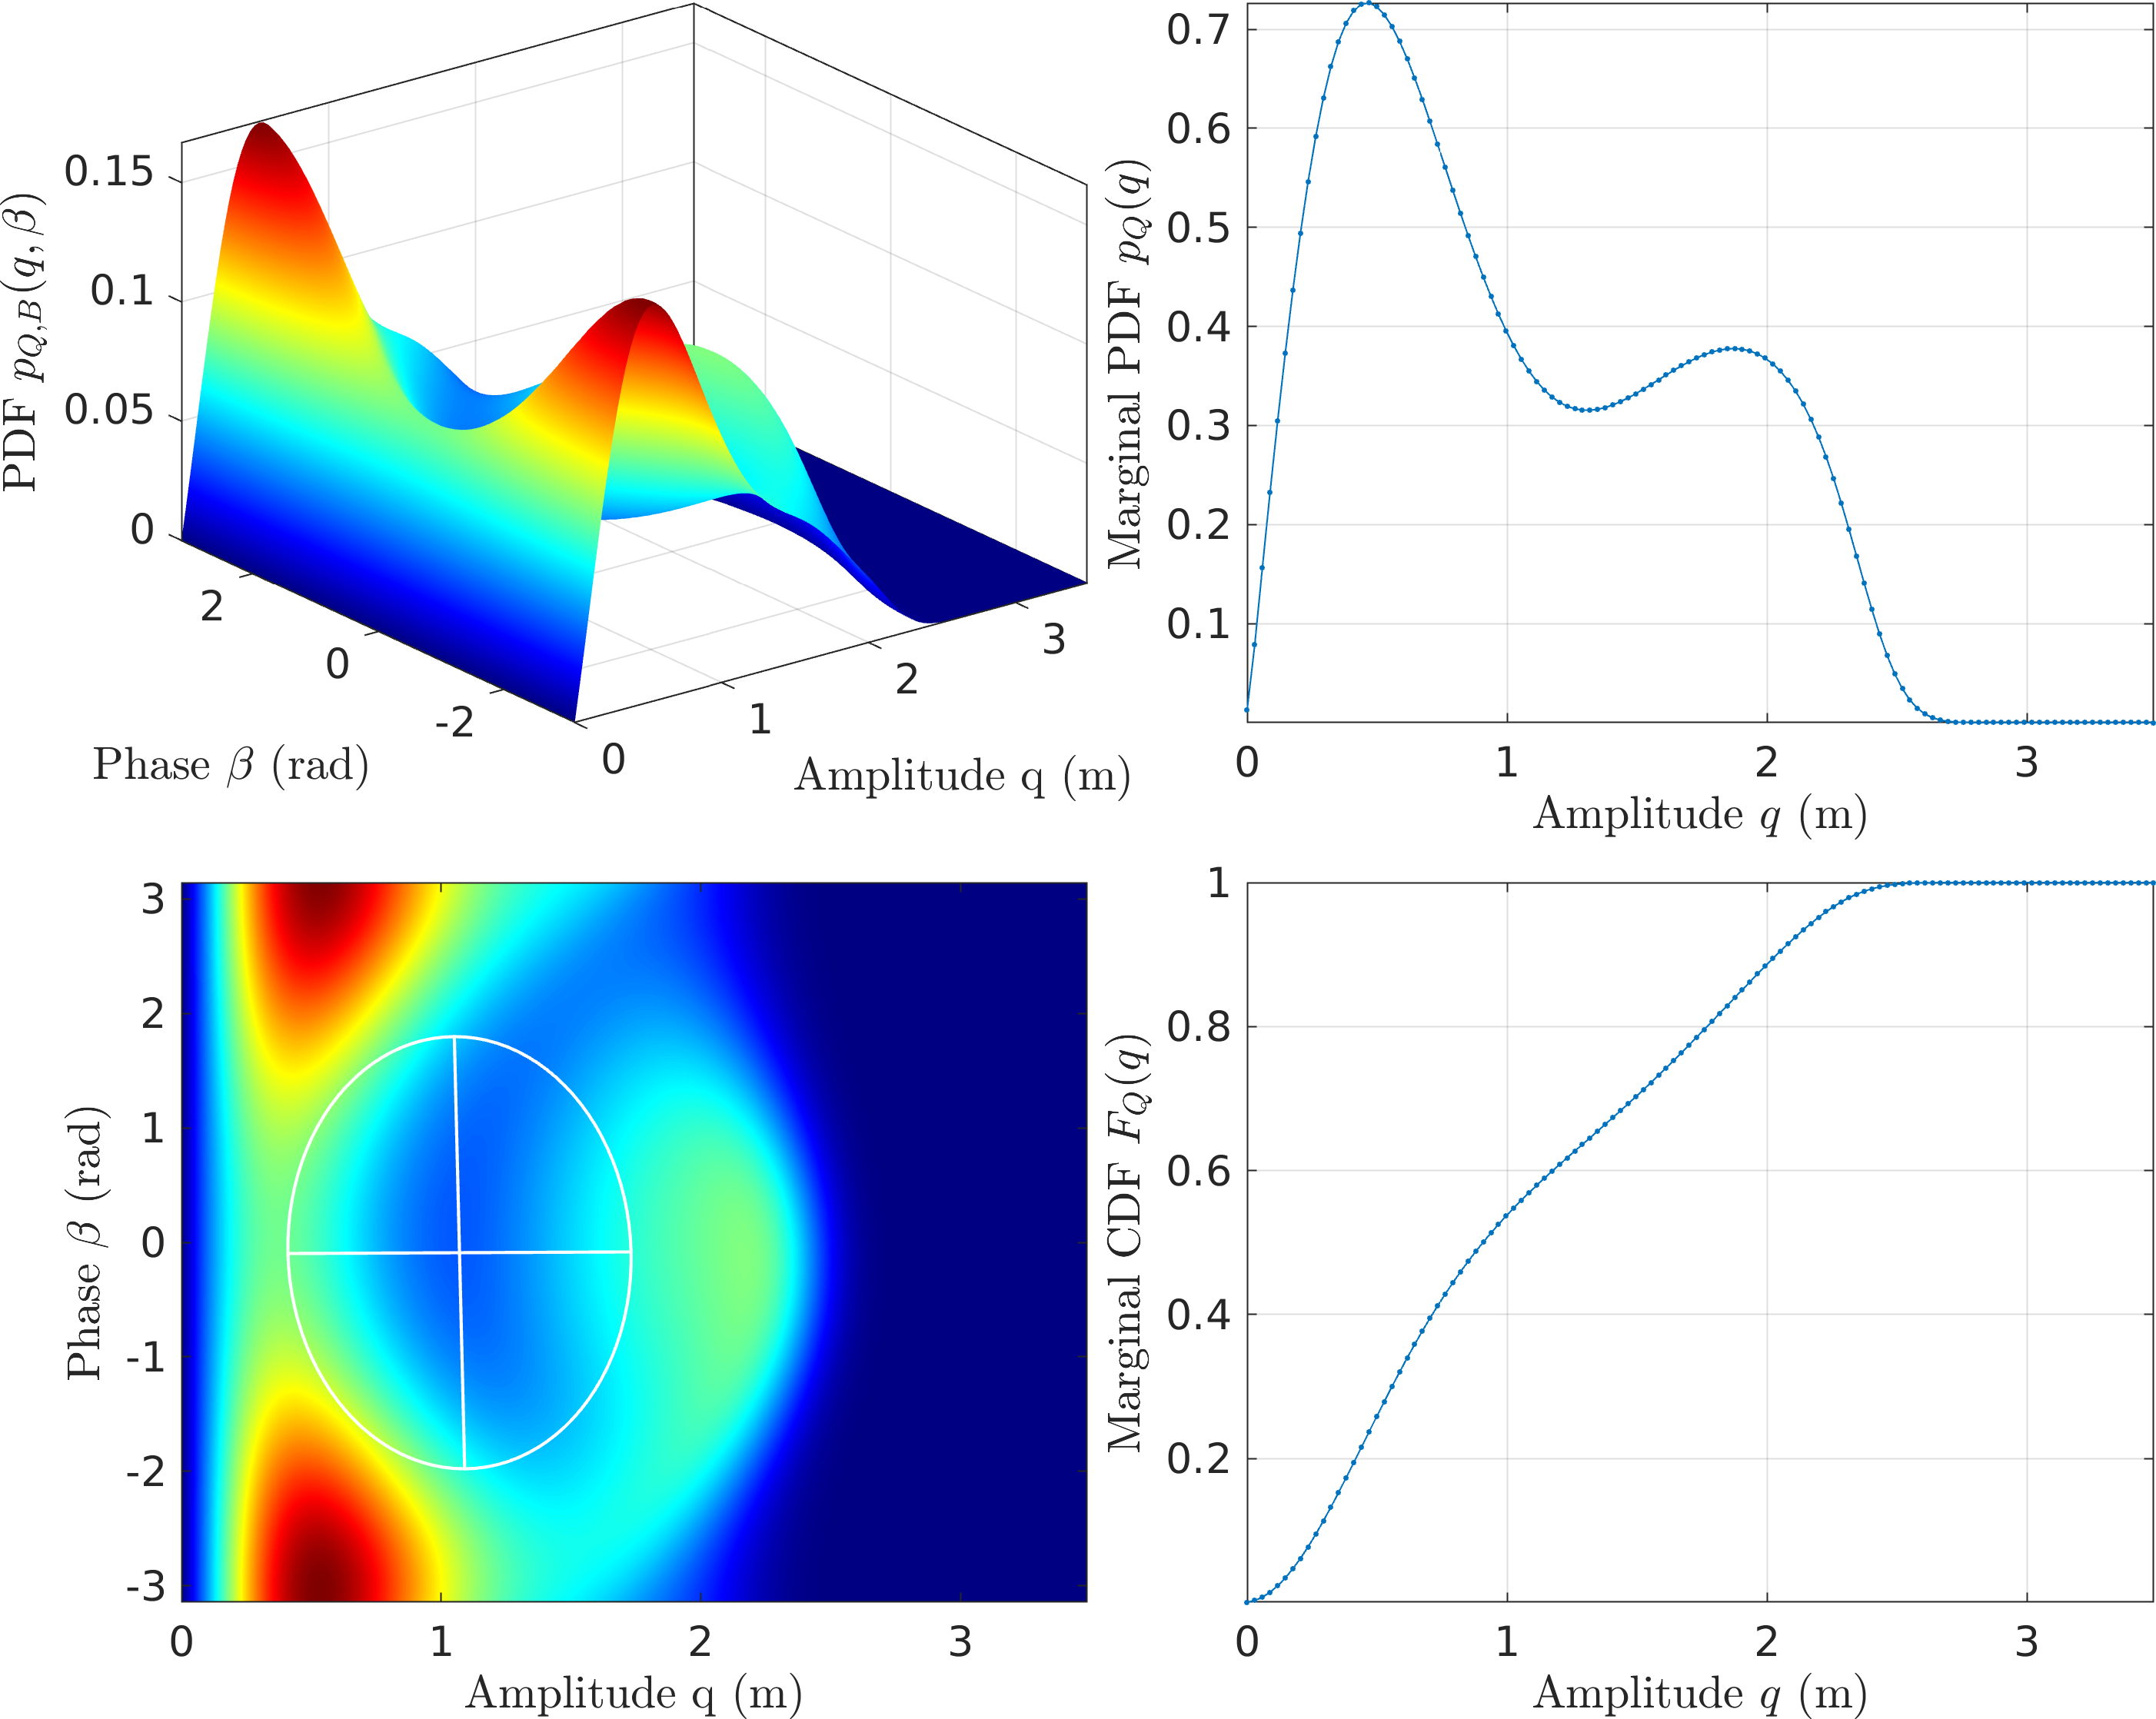
\includegraphics[width=.9\linewidth]{FIGS/G3_SDOFFPE_duffing_emms1.png}
\caption{FPE Results for the Duffing Oscillator with CXA (EMMS1)}
\end{figure}
\end{figure}
\item \(\mathcal{O}(\textcolor{red}{p^2})\) EMMS
\label{sec:org625c676}
\begin{figure}
\begin{figure}[htbp]
\centering
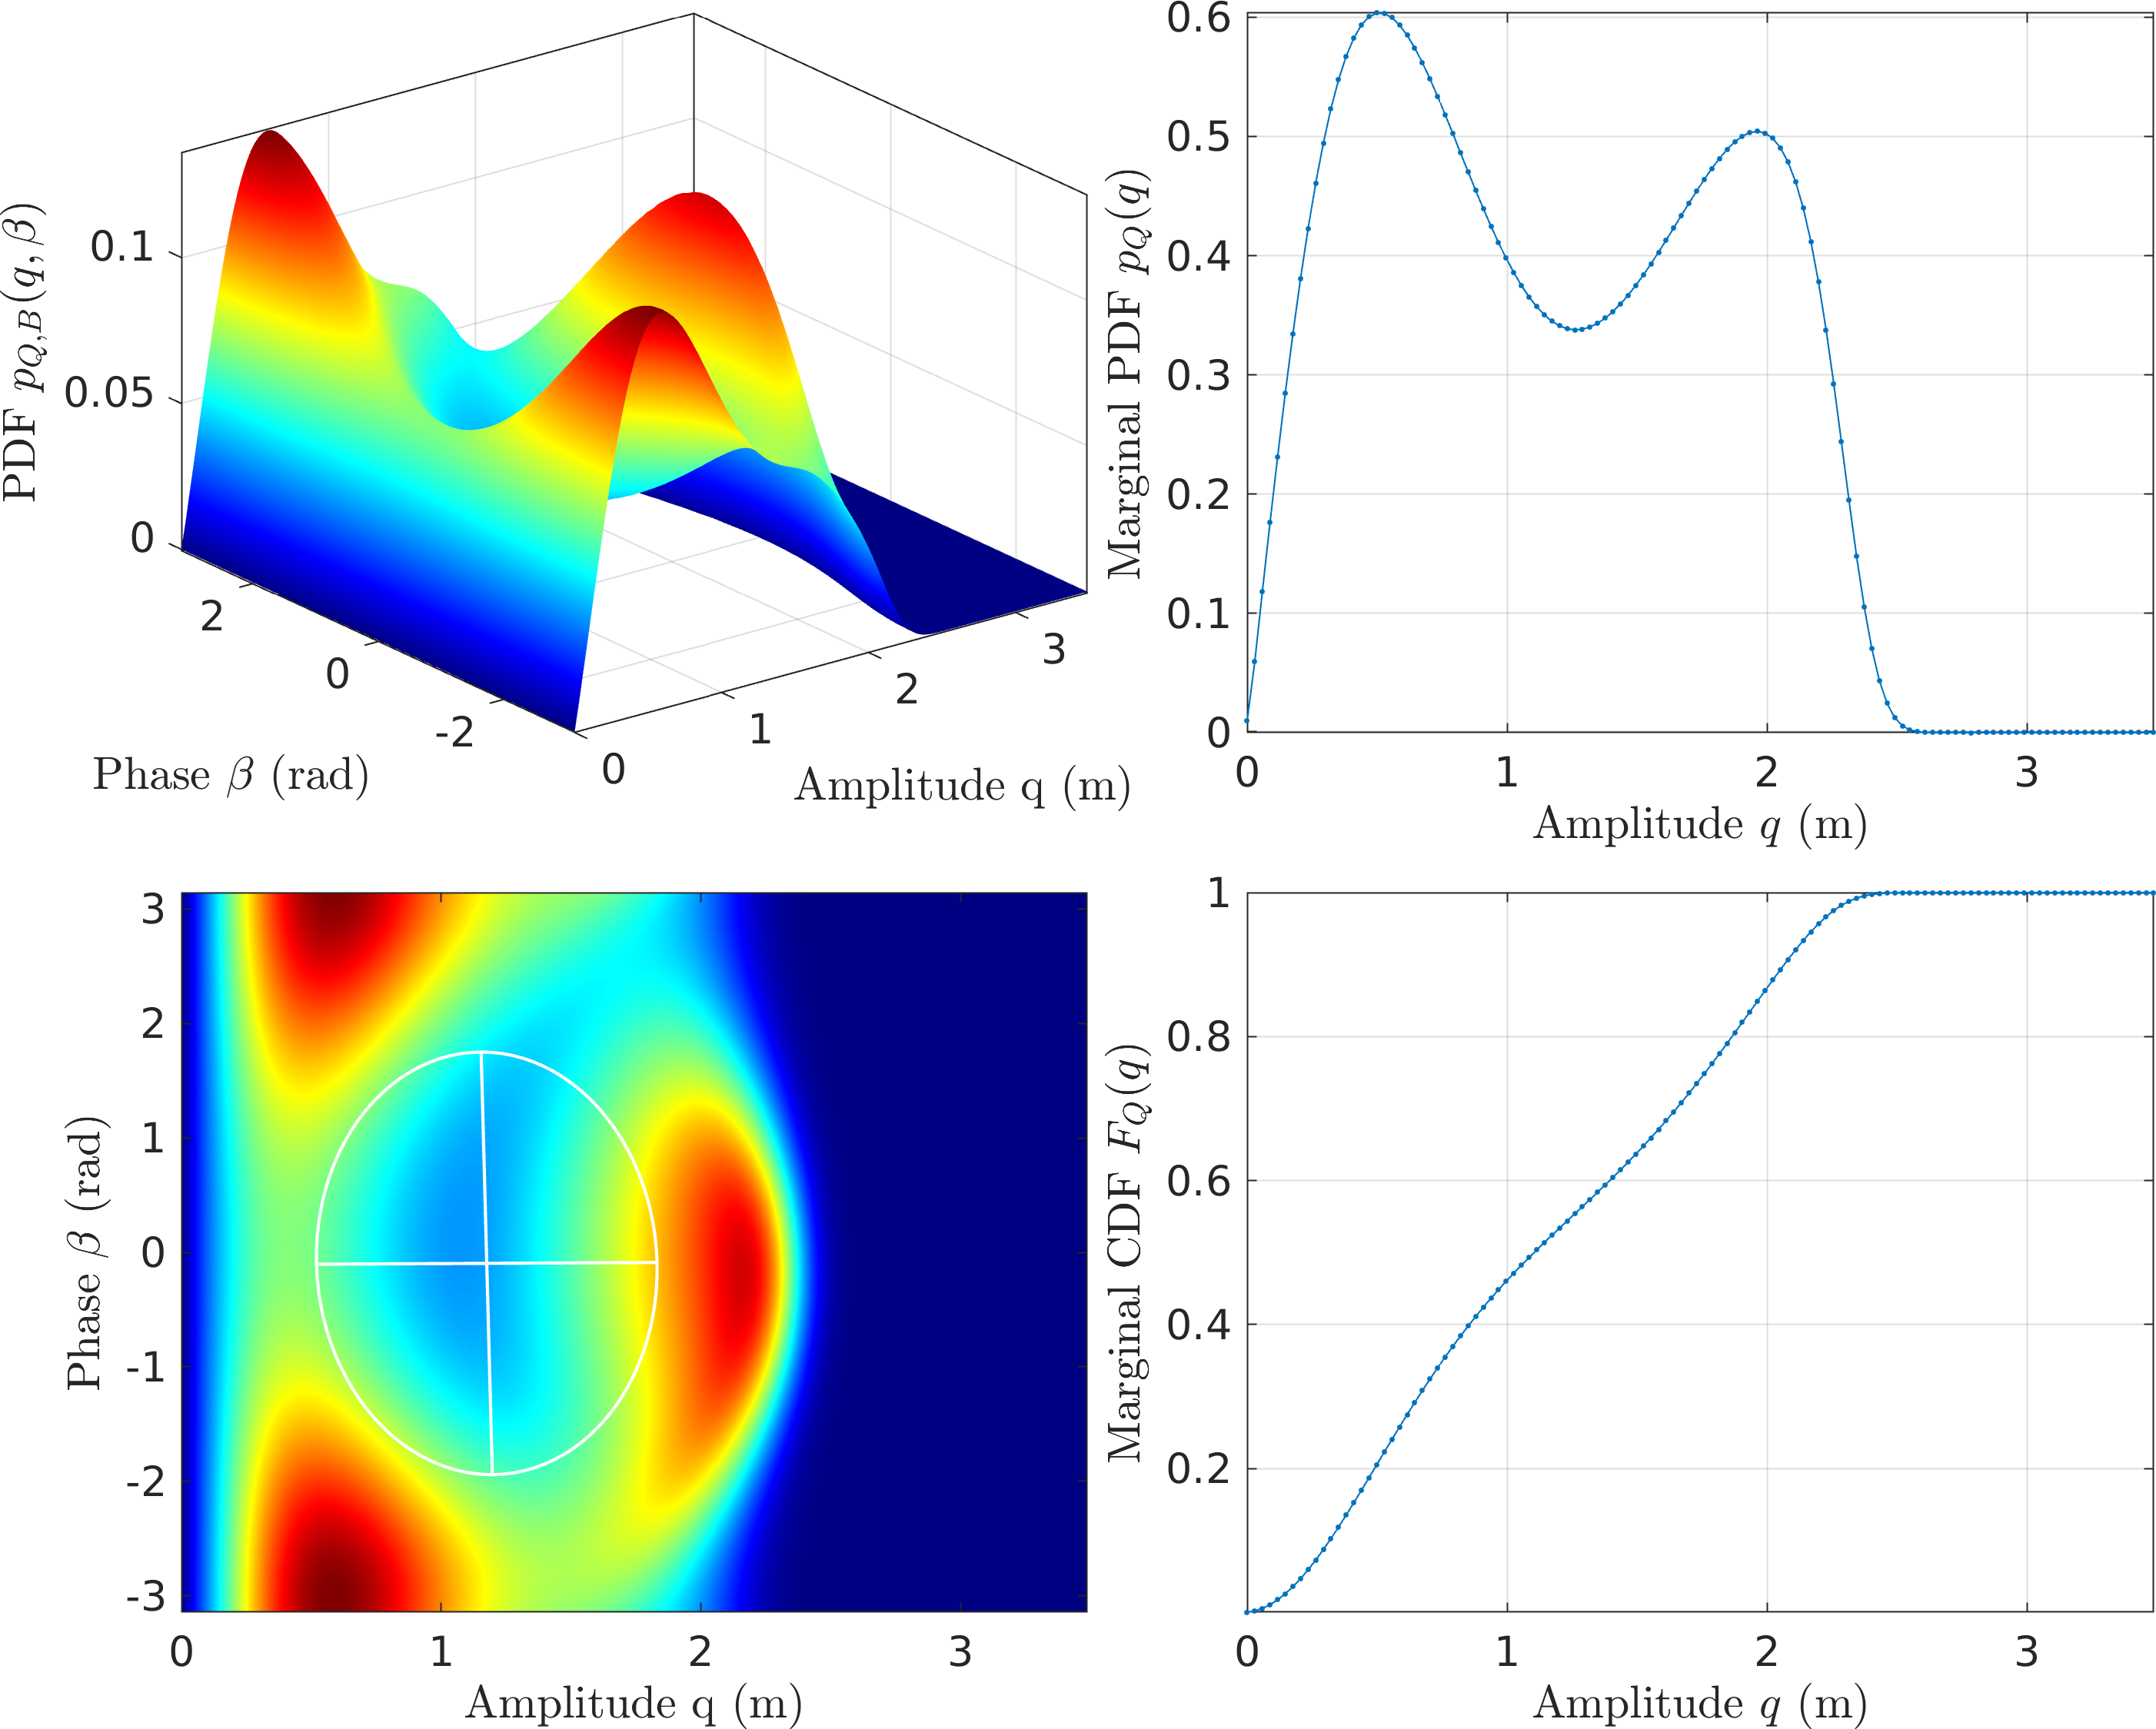
\includegraphics[width=.9\linewidth]{FIGS/G3_SDOFFPE_duffing_emms2.png}
\caption{FPE Results for the Duffing Oscillator with CXA (EMMS2)}
\end{figure}
\end{figure}
\end{enumerate}
\subsubsection{SDOF Oscillator with Friction}
\label{sec:org79e5133}
\begin{itemize}
\item Considered EOM:
$$ \ddot{x} + 2\zeta_n\omega_n \dot{x}+\omega_n^2x + f_{jenk}(x; k_t, \mu N)=F\cos\sigma, $$
with parameters,
$$ \omega_0=1\,rad/s,\quad \zeta_n=10^{-3},\quad k_t=3\,N/m,\quad \mu N=0.5\,N,\quad F=0.2\,N. $$
\item Used EPMC to compute the backbones first
\begin{figure}
\begin{figure}[htbp]
\centering
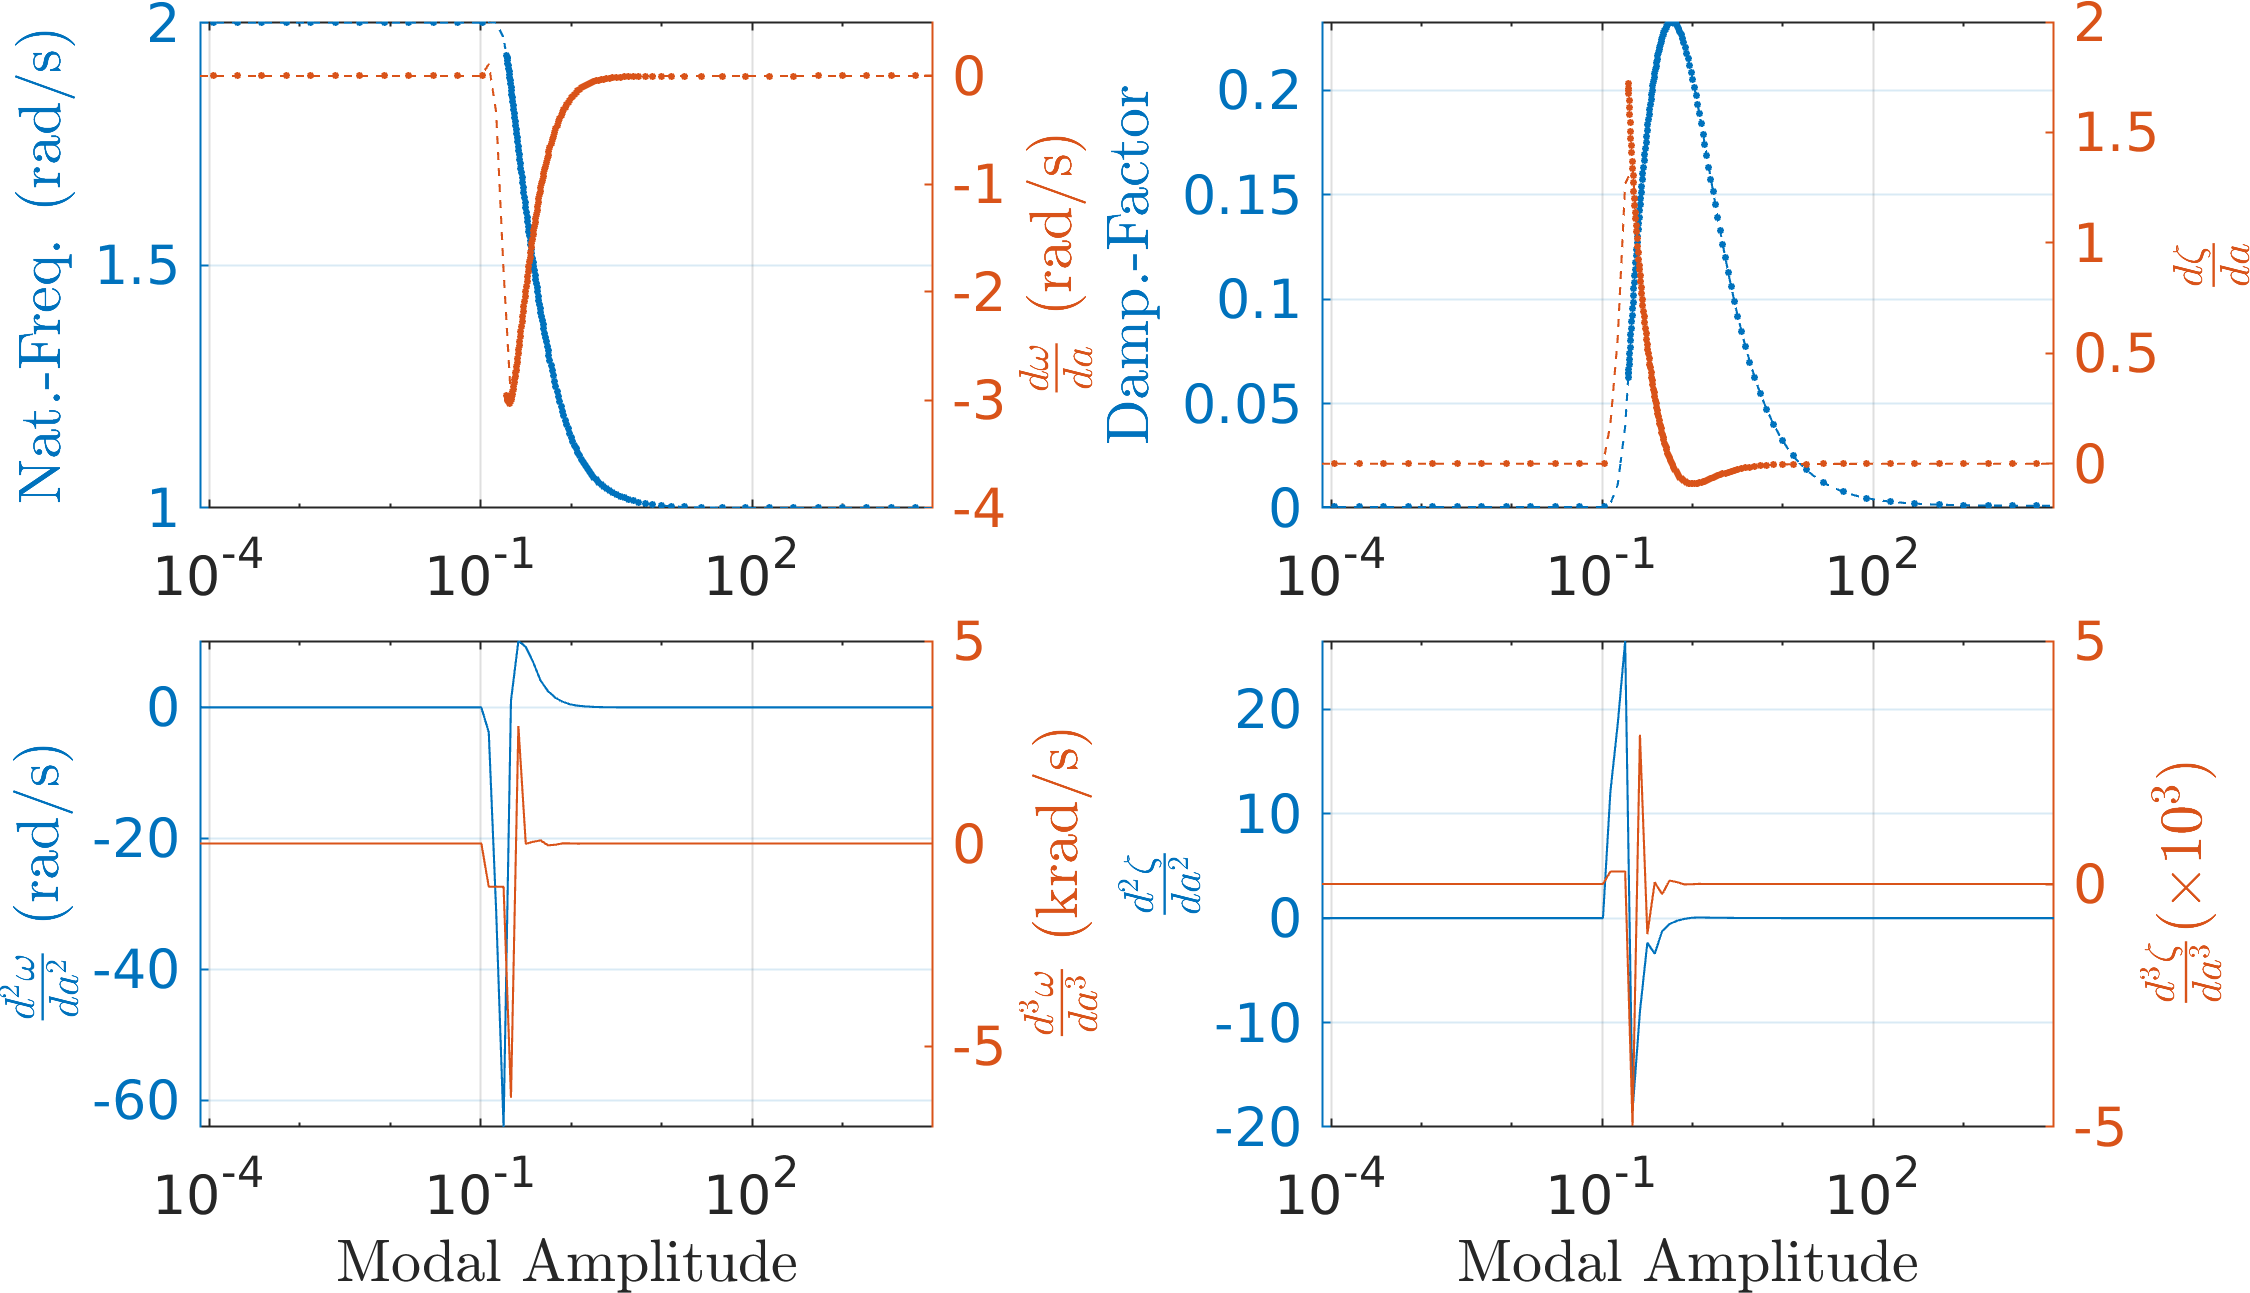
\includegraphics[width=.9\linewidth]{FIGS/G1_SDOFEPMC_jenkins.png}
\caption{EPMC Backbone for the SDOF Duffing oscillator}
\end{figure}
\end{figure}
\item This is next used to obtain the PDF of the slow flow system using the four different formulations. Here is a summary.

\item Both the first order approximations seem to result in spurious oscillations in the predicted PDF. The second order forms seem to find it easier.
Perhaps this is related to the interpolated approximation of the non-smooth backbone?
\end{itemize}
\begin{enumerate}
\item \(\mathcal{O}(\textcolor{red}{\epsilon})\) MMS
\label{sec:org56effe7}
\begin{figure}
\begin{figure}[htbp]
\centering
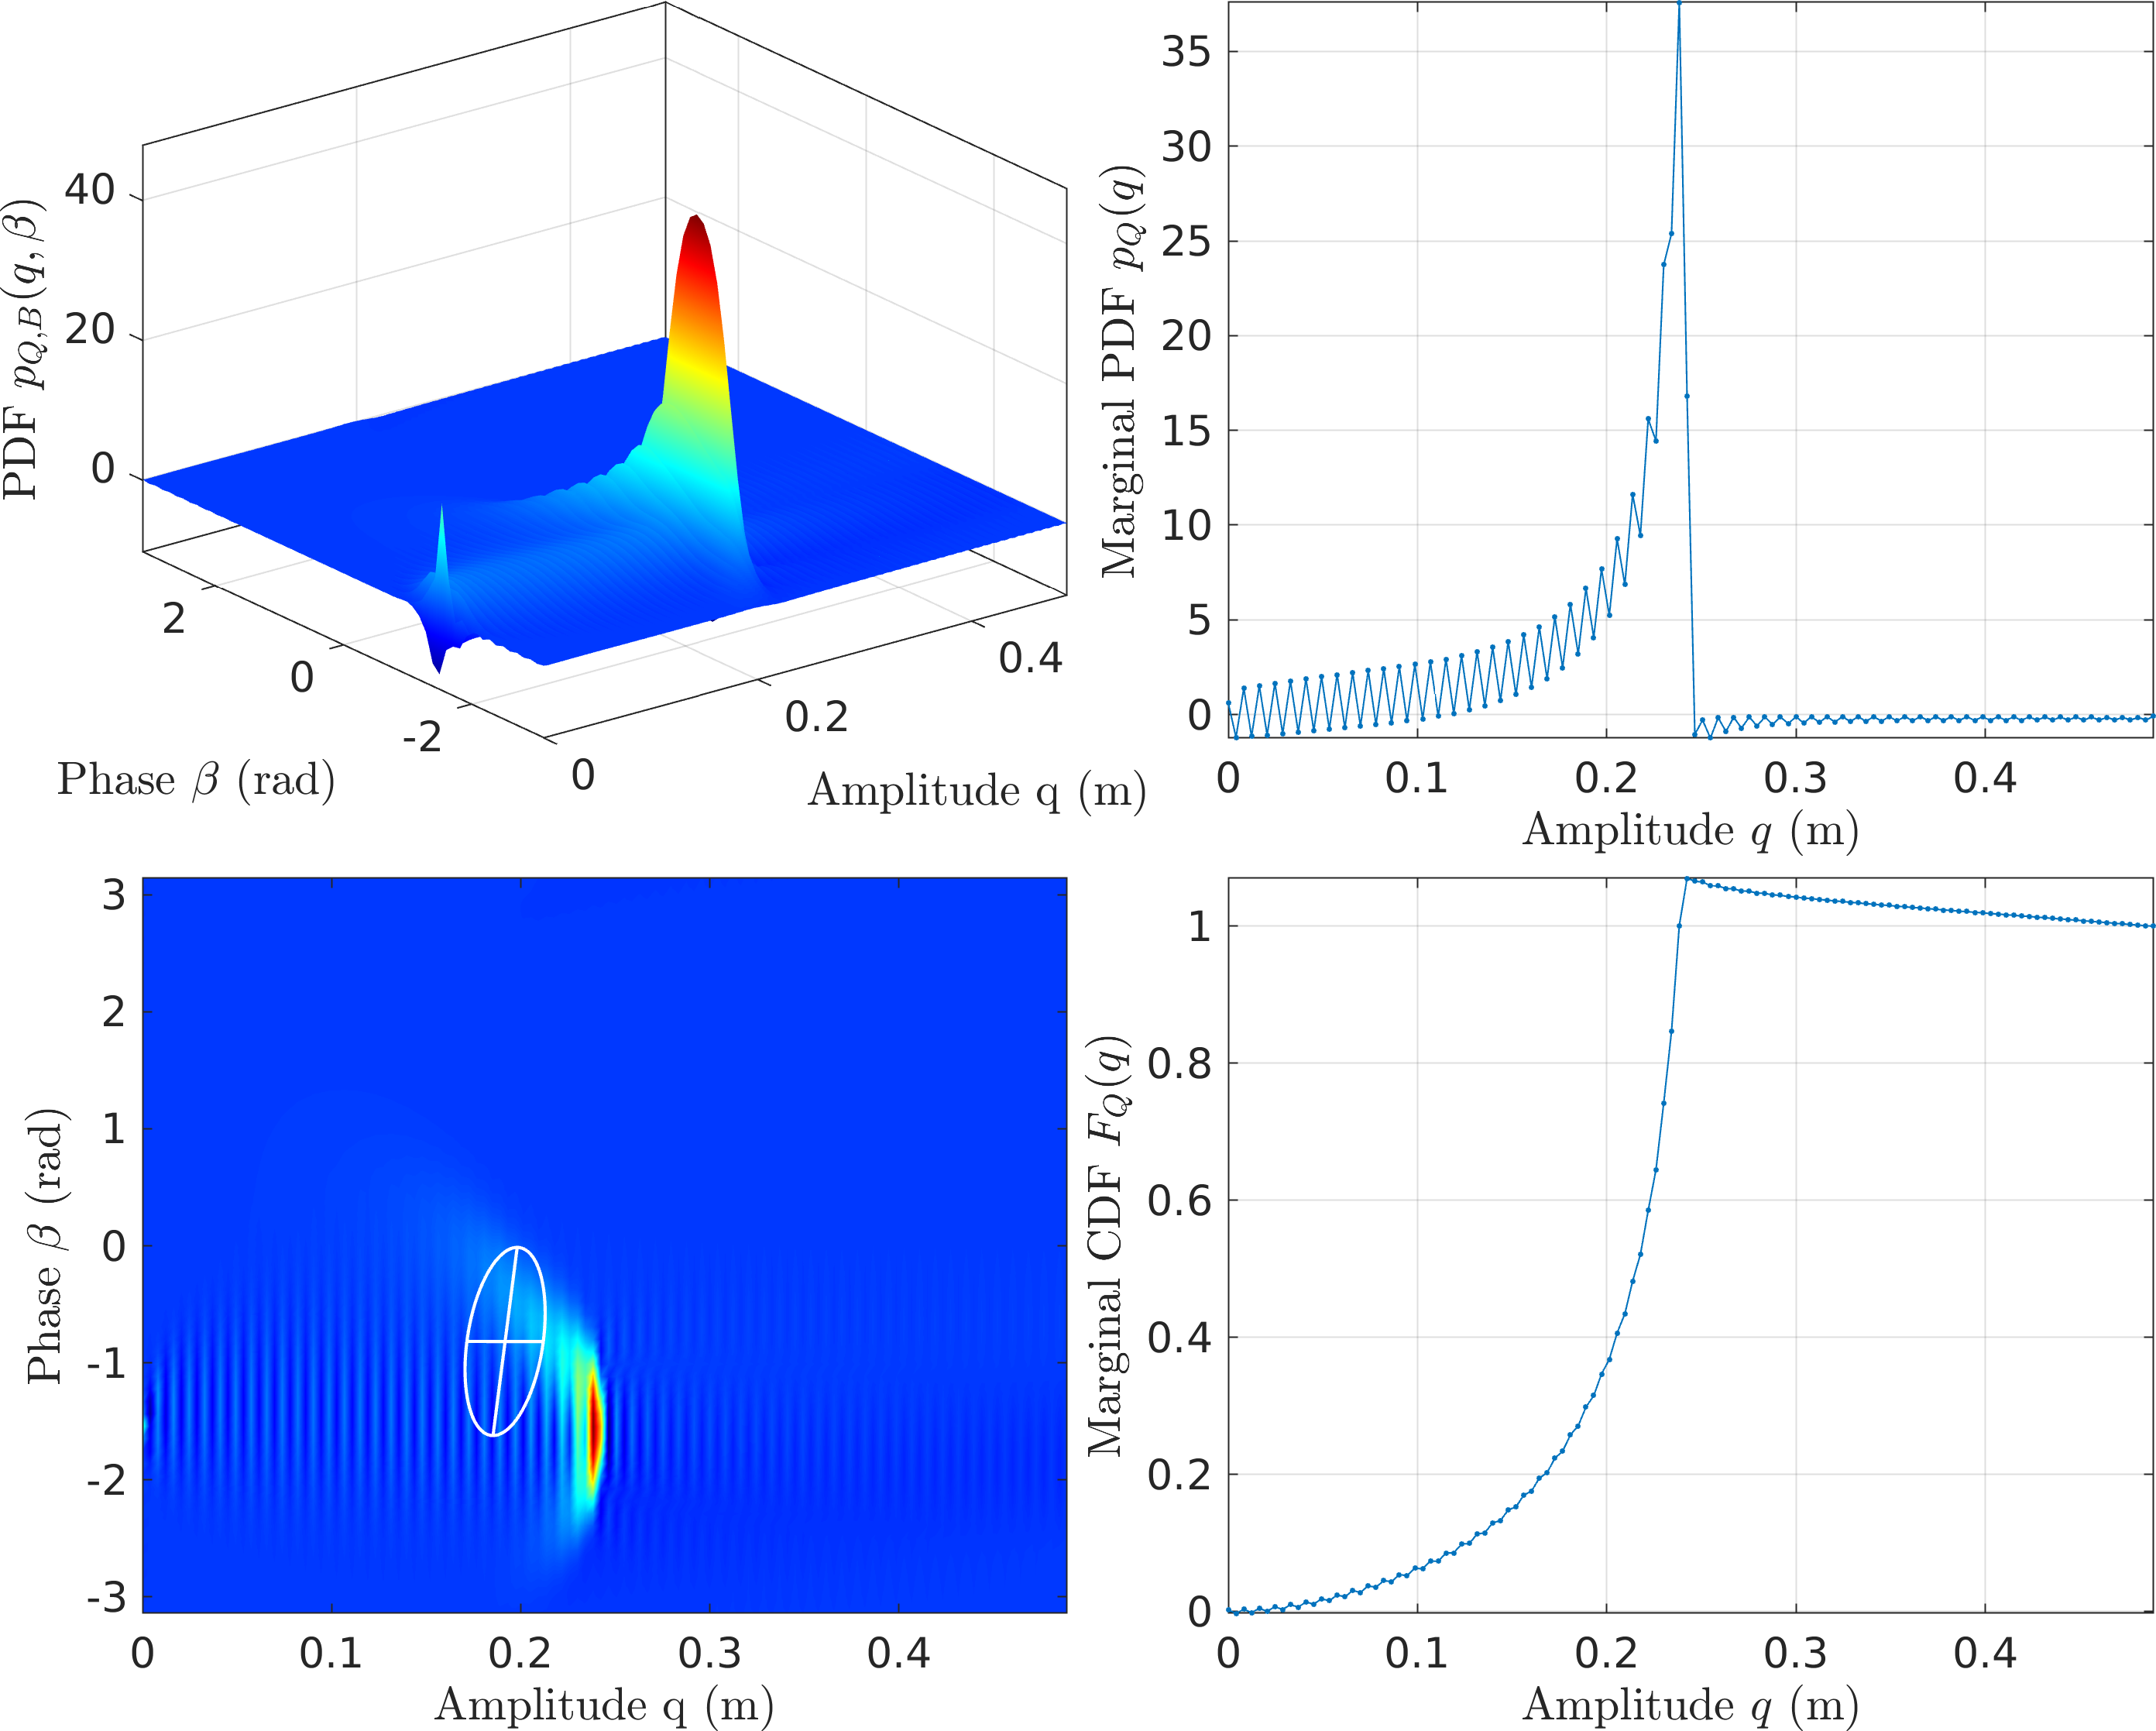
\includegraphics[width=.9\linewidth]{FIGS/G3_SDOFFPE_jenkins_mms1.png}
\caption{FPE Results for the Frictional Oscillator with MMS1}
\end{figure}
\end{figure}
\item \(\mathcal{O}(\textcolor{red}{\epsilon^2})\) MMS
\label{sec:org75a84f6}
\begin{figure}
\begin{figure}[htbp]
\centering
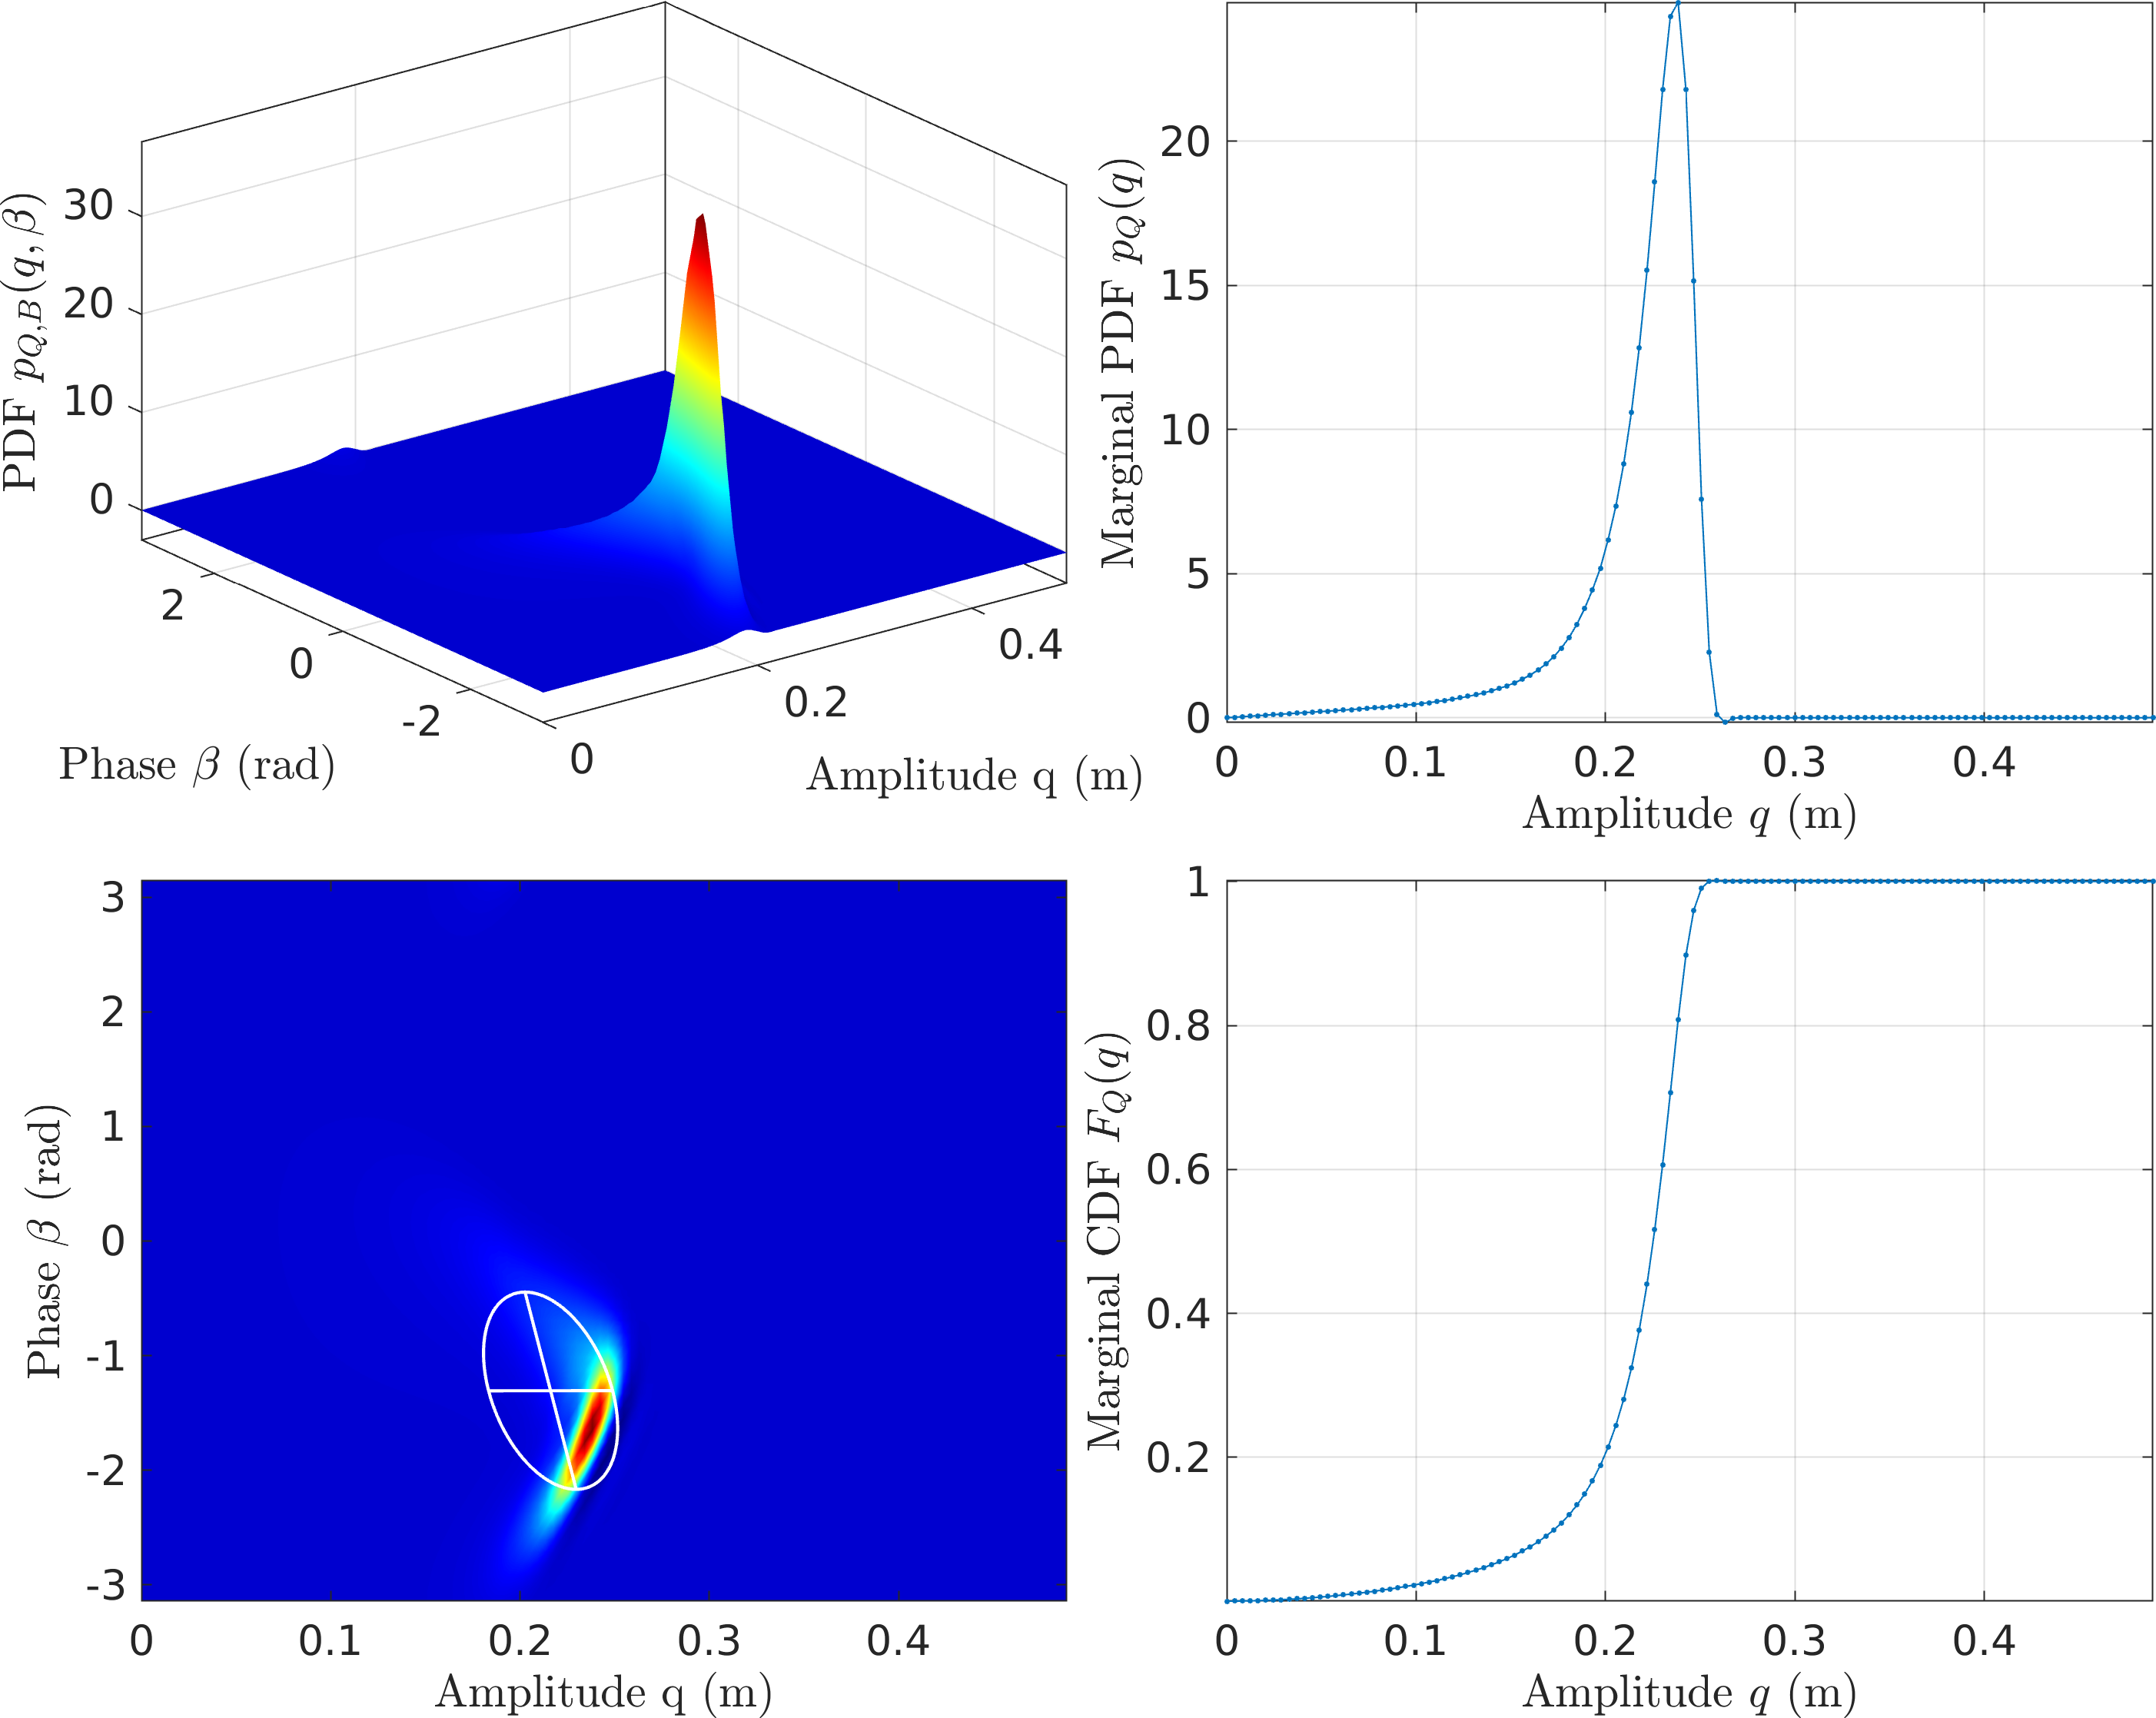
\includegraphics[width=.9\linewidth]{FIGS/G3_SDOFFPE_jenkins_mms2.png}
\caption{FPE Results for the Frictional Oscillator with MMS2}
\end{figure}
\end{figure}
\item CXA (\(\mathcal{O}(\textcolor{red}{p})\) EMMS)
\label{sec:org44e78b1}
\begin{figure}
\begin{figure}[htbp]
\centering
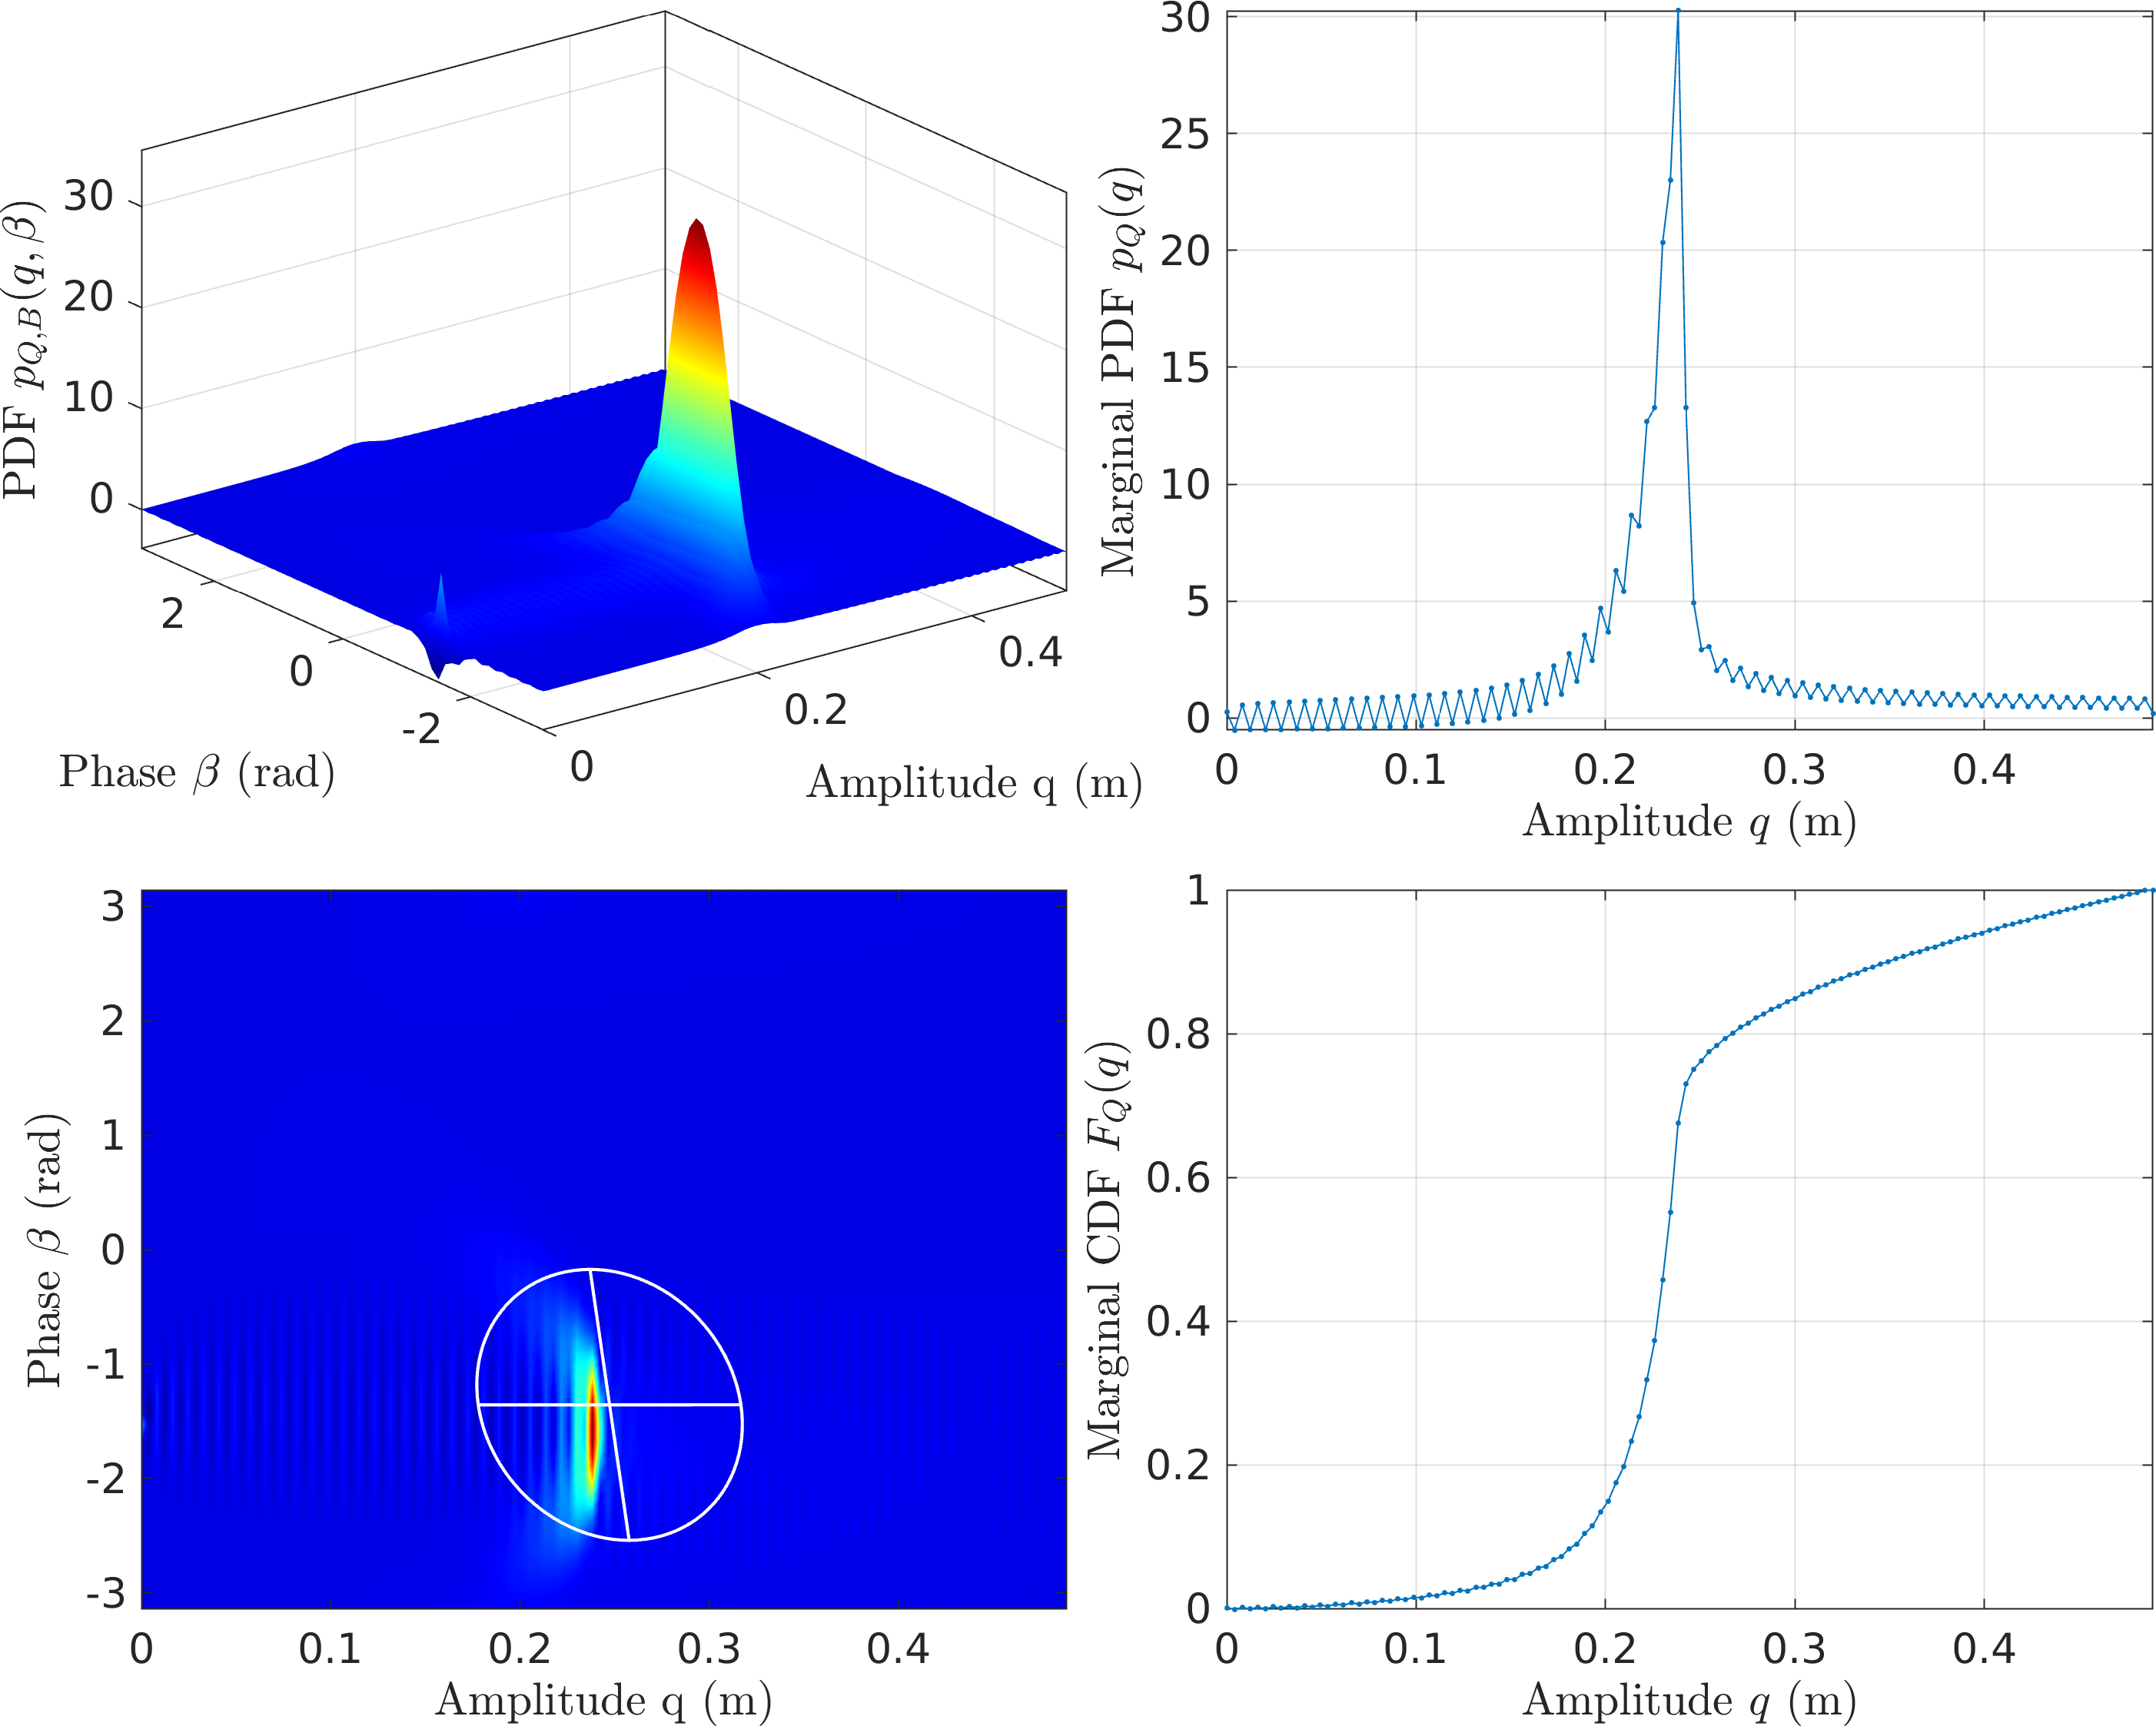
\includegraphics[width=.9\linewidth]{FIGS/G3_SDOFFPE_jenkins_emms1.png}
\caption{FPE Results for the Frictional Oscillator with CXA (EMMS1)}
\end{figure}
\end{figure}
\item \(\mathcal{O}(\textcolor{red}{p^2})\) EMMS
\label{sec:org619cc79}
\begin{figure}
\begin{figure}[htbp]
\centering
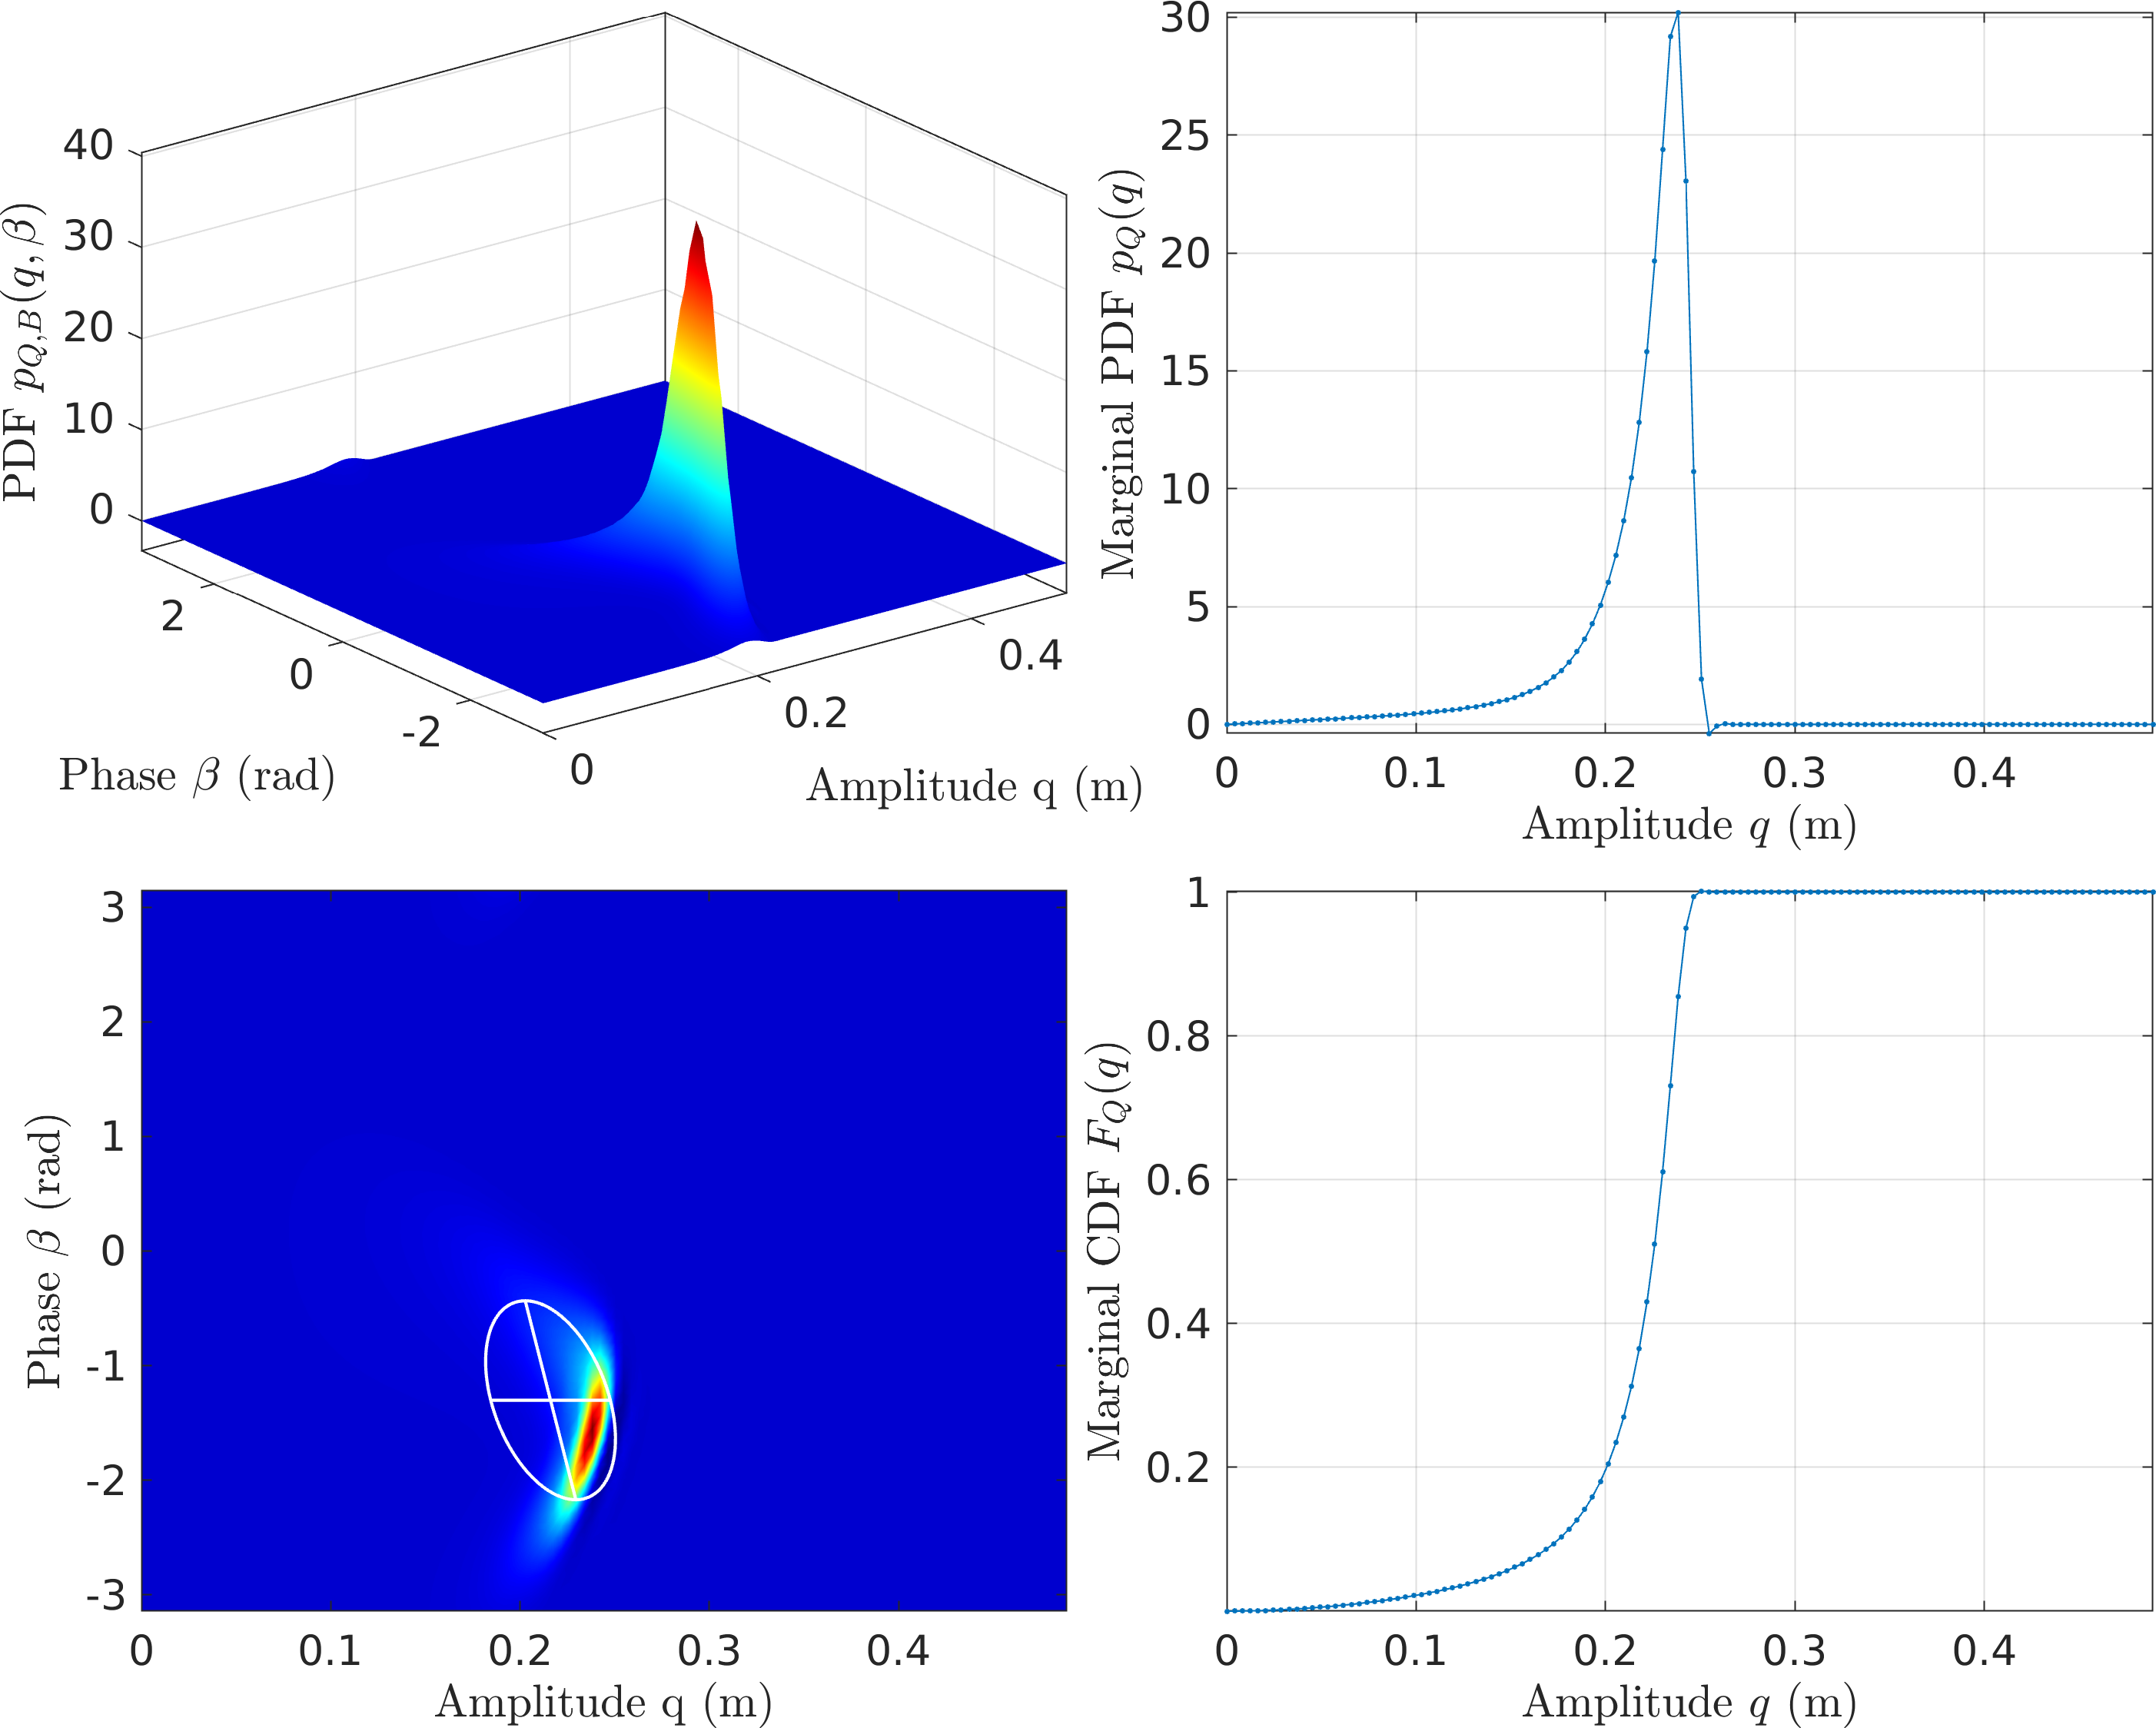
\includegraphics[width=.9\linewidth]{FIGS/G3_SDOFFPE_jenkins_emms2.png}
\caption{FPE Results for the Frictional Oscillator with CXA (EMMS2)}
\end{figure}
\end{figure}
\end{enumerate}
\subsubsection{Pointers from Tobi on Experimentation}
\label{sec:org917f6d4}
\begin{itemize}
\item If we have a Gaussian process with a given target PSD that needs to be achieved for the force, this can be done iteratively.
\item What we have here is,
\begin{itemize}
\item PSD:
$$ \Phi_{FF}(\omega) = \frac{\lambda^2\overline{\nu}^2}{4\pi} \frac{\overline{\Omega}^2+\frac{\overline{\nu}^4}{4}+\omega^2}{(\Omega^2+\frac{\overline{\nu}^4}{4}-\omega^2)^2+\omega^2\overline{\nu}^4}\text{, with } \overline{\nu}=\frac{\nu}{\sqrt{F_s}}.  $$
\item PDF:
\begin{equation*}
  p_F(f) = \begin{cases} \frac{1}{\pi\sqrt{(\Omega^2-f^2)}} & |f|< F\\
    0 & \text{otherwise} \end{cases}
\end{equation*}
\end{itemize}
\item If we generated a voltage signal \(v(t) = V\cos\sigma\) with random phase \(\sigma\), we don't have enough degrees of freedom to adjust the force spectrum.
\item We discussed 2 alternatives:
\end{itemize}
\begin{enumerate}
\item Set \(\sigma=0\) and make \(F\) a stationary Gaussian process with desired spectrum
\label{sec:org829d1d8}
\begin{itemize}
\item This allows Tobi to apply techniques he is already familiar with
\item The excitation is not phase-noise excitation
\item Amplitude-phase equations are still applicable but the will look different
\end{itemize}
\item Try a novel iterative approach
\label{sec:org702c073}
\begin{itemize}
\item We start with providing a desired PSD to the excitation
\item We take the output voltage in time domain and tranform it to the desired PDF
\item We then check the output force spectrum and adjust the initial PSD accordingly
\item Tobi is not sure if this has been tried in the literature, said he'll try to find papers
\item This will be a new approach from the experimental side.
\end{itemize}
\end{enumerate}
\subsubsection{Things to try}
\label{sec:org670a140}
\begin{itemize}
\item Linear interpolation
\item DG for discretization
\end{itemize}
\section{References}
\label{sec:orge162bb6}
\hypertarget{citeproc_bib_item_1}{[1] M. F. Dimentberg, E. Mo, and A. Naess, “Probability Density and Excursions of Structural Response to Imperfectly Periodic Excitation,” \textit{Journal of engineering mechanics}, vol. 133, no. 9, pp. 1037–1041, Sep. 2007, doi: \href{https://doi.org/10.1061/(ASCE)0733-9399(2007)133:9(1037)}{10.1061/(ASCE)0733-9399(2007)133:9(1037)}.}

\hypertarget{citeproc_bib_item_2}{[2] W. Eugene and Z. Moshe, “On the relation between ordinary and stochastic differential equations,” \textit{International journal of engineering science}, vol. 3, no. 2, pp. 213–229, Jul. 1965, doi: \href{https://doi.org/10.1016/0020-7225(65)90045-5}{10.1016/0020-7225(65)90045-5}.}

\hypertarget{citeproc_bib_item_3}{[3] A. Naess and V. Moe, “Efficient path integration methods for nonlinear dynamic systems,” \textit{Probabilistic engineering mechanics}, vol. 15, no. 2, pp. 221–231, Apr. 2000, doi: \href{https://doi.org/10.1016/S0266-8920(99)00031-4}{10.1016/S0266-8920(99)00031-4}.}

\hypertarget{citeproc_bib_item_4}{[4] F. Hu, L. Chen, and W. Zhu, “Stationary response of strongly non-linear oscillator with fractional derivative damping under bounded noise excitation,” \textit{International journal of non-linear mechanics}, vol. 47, no. 10, pp. 1081–1087, Dec. 2012, doi: \href{https://doi.org/10.1016/j.ijnonlinmec.2011.09.012}{10.1016/j.ijnonlinmec.2011.09.012}.}\bigskip
\end{document}